\documentclass[conference]{IEEEtran}
\IEEEoverridecommandlockouts

\usepackage{cite}
\usepackage{amsmath,amssymb,amsfonts}
\usepackage{graphicx}
\usepackage{textcomp}
\usepackage{xcolor}
\usepackage{url}
\usepackage{booktabs}

\begin{document}

\title{A Machine Learning-Driven Visual Analytics Framework for \\ Probabilistic Housing Pressure Forecasting}

\author{
\IEEEauthorblockN{Peidong Wang}
\IEEEauthorblockA{
EMATM0066 – Visual Analytics 2025\\
University of Bristol}
}

\maketitle

\begin{abstract}
This study presents a visual analytics framework driven by machine learning to explore structural housing pressure across local authorities in England and Wales using Census data from 2011 and 2021\cite{noauthor_census_nodate}. The analysis focuses on overcrowding as a key indicator of housing stress. It examines how overcrowding relates to housing tenure, rental dependency, and high-density accommodation patterns.

Data from both census years were combined at the local authority level using six main housing indicators: home ownership, private renting, social renting, overcrowding, flat-based housing, and shared accommodation. Missing values caused by geographic differences were handled with Bayesian imputation, which significantly improved data reliability over baseline methods\cite{davidson-pilon_bayesian_2016}.

To uncover hidden socio-economic structures, K-Means clustering identified four housing archetypes\cite{macqueen_methods_nodate}. Dimensionality reduction followed, using PCA and t-SNE to reveal strong structural differences among regions\cite{lee_generalized_nodate, maaten_visualizing_2008}. A Bayesian forecasting model then estimated overcrowding pressure for 2031, including uncertainty intervals for policy implications.

Results indicate a notable shift from ownership-based housing systems to rental dependency and high-density living. This study shows how combining visual analytics with Bayesian modeling can aid in understanding socio-economic policies with awareness of uncertainty.
\end{abstract}

\begin{IEEEkeywords}
Housing Pressure, Visual Analytics, Bayesian Inference, Census Data, Socio-Economic Drivers, Urban Planning, PCA, t-SNE, K-Means
\end{IEEEkeywords}

\section{Introduction}
Housing pressure has become one of the biggest social and economic challenges in England and Wales. This issue is especially pronounced in urban areas where affordability, reliance on rentals, and overcrowding are growing worse. Although housing supply has increased in many parts, the quality and accessibility of housing vary greatly. Standard statistics often miss the deeper connections between changes in housing tenure, residential density, and the risk of long-term overcrowding.

Among these issues, overcrowding stands out as a critical indicator. It shows both economic inequality and barriers to housing access. High levels of overcrowding usually link to low home ownership, the rapid growth of the private rental market, and a greater reliance on high-density housing like flats and converted properties. These trends are not only uneven across different regions but also persist over time.

The primary users of this visualization are policy analysts, local government planners, and housing researchers. They need clear evidence to understand long-term housing pressure. Instead of focusing on short-term reports, these users need tools that allow for exploration of data, discovery of patterns, and forecasting that considers uncertainty.

This project creates a visual analytics framework to study how housing structures changed between the 2011 and 2021 Census and how these changes might affect future housing pressure by 2031. The analysis uses statistical modeling, dimensionality reduction, clustering, and Bayesian forecasting, all within a combined Tableau dashboard.

The main research questions are:
\begin{enumerate}
    \item How has overcrowding changed from 2011 to 2021 across local authorities?
    \item What structural relationships exist between overcrowding, declines in ownership, and growth in the rental market?
    \item Can local authorities be categorized into understandable housing archetypes through projection-based analysis?
    \item Which regions are expected to experience the highest housing pressure by 2031 according to Bayesian forecasting?
\end{enumerate}

To address these questions, the study employs Bayesian imputation for missing values, K-Means clustering for social and economic segmentation, PCA and t-SNE for reducing dimensions, and Bayesian Ridge Regression for predicting future overcrowding. The aim is not just to visualize the current housing situation, but also to aid more informed decision-making through clear probabilistic forecasts.

\begin{figure}[htbp]
    \centering
    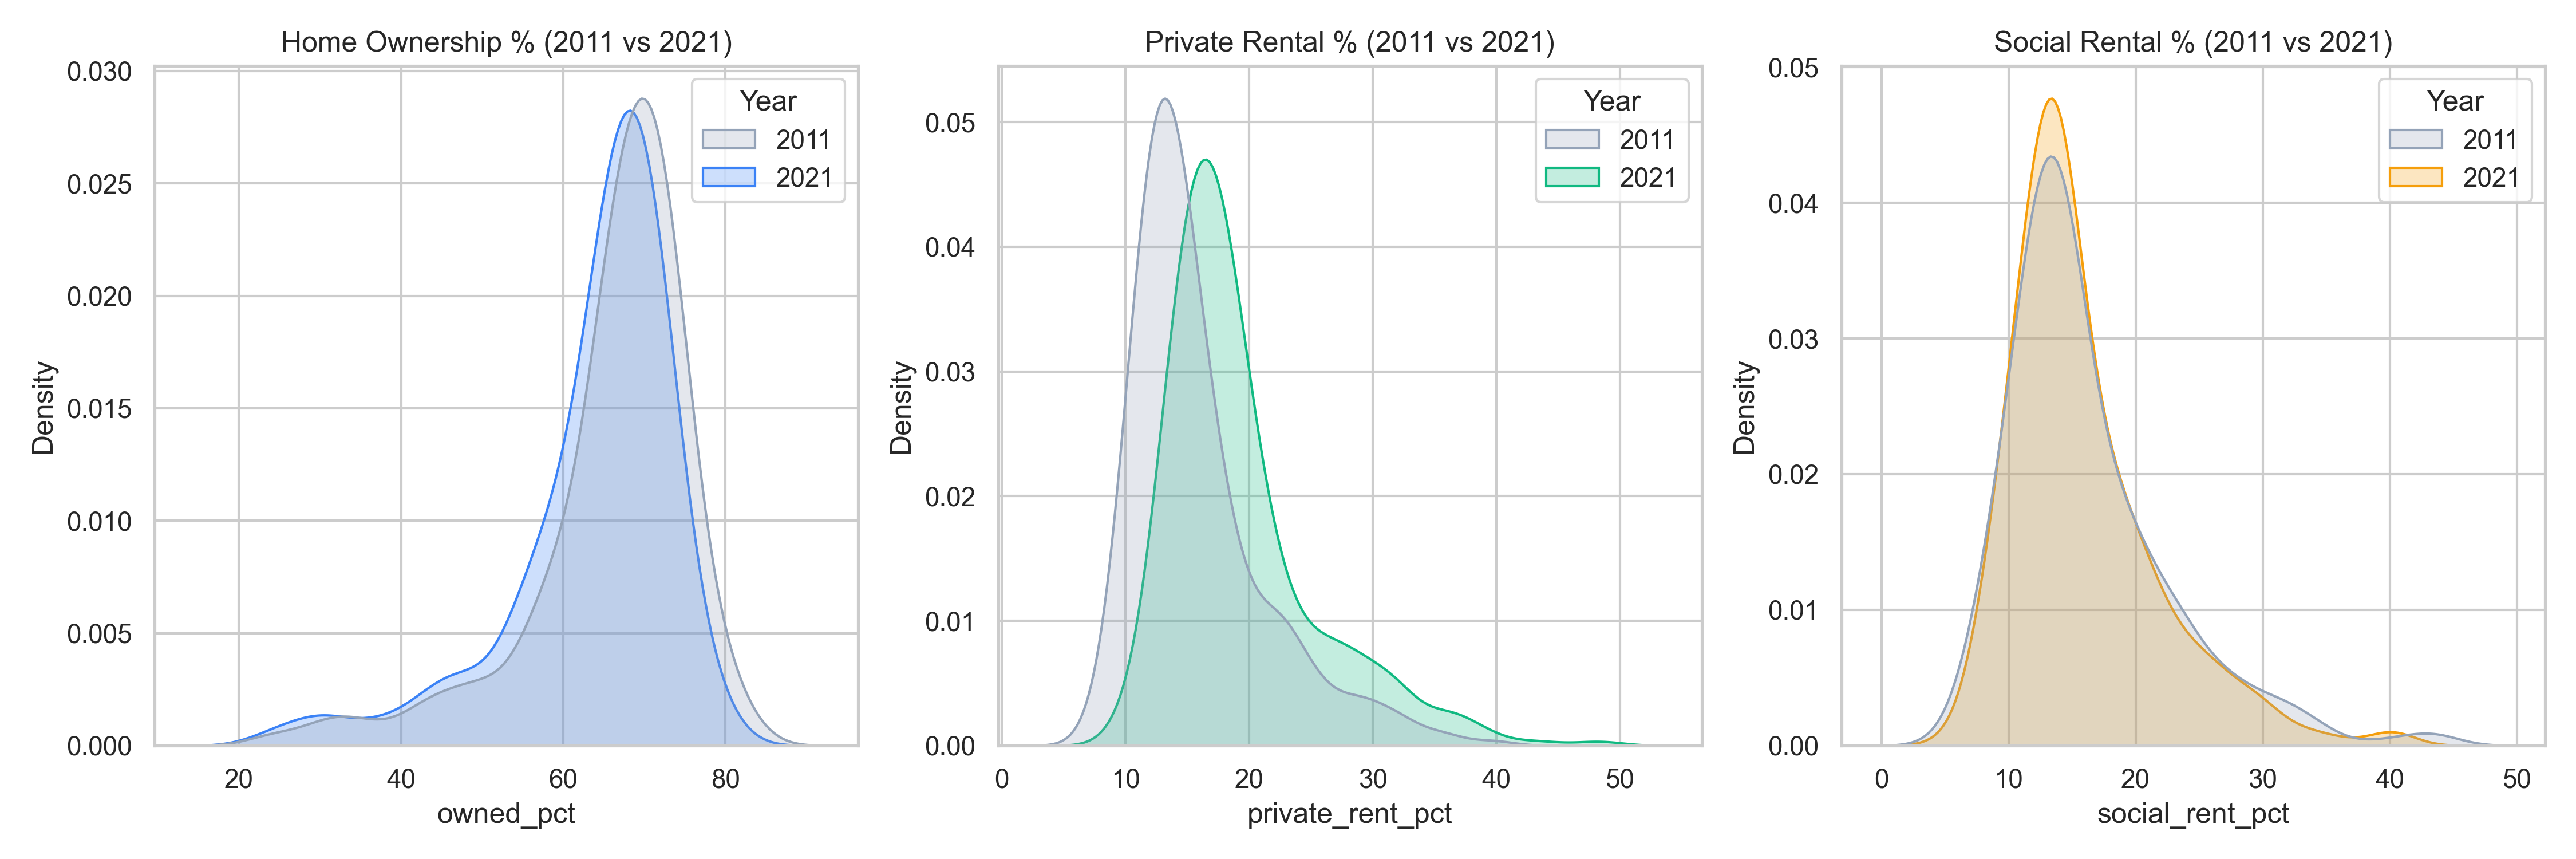
\includegraphics[width=0.48\textwidth]{figures/eda_tenure_shifts.png}
    \caption{Decadal Tenure Shifts (2011 vs 2021): Density plots illustrating the redistribution of home ownership, private rental, and social rental sectors across 331 Local Authorities.}
    \label{fig:tenure_shifts}
\end{figure}


\section{Data Preparation}

\subsection{Data Sources}
This study uses official census data from the 2011 and 2021 Census of England and Wales to analyse structural housing pressure at the Local Authority (LA) level. The objective is to compare long-term changes in housing conditions and identify regions at risk of future overcrowding.

Following the coursework requirements, three datasets were selected from the 2011 Census and one corresponding topic group from the 2021 Census. The selected variables were chosen because they directly reflect housing accessibility, tenure transition, and residential density.

\subsubsection{2011 Census Tables}
The following tables were used:
\begin{itemize}
    \item \textbf{KS402EW} -- Tenure
    \item \textbf{QS408EW} -- Occupancy Rating (Rooms)
    \item \textbf{QS401EW} -- Accommodation Type
\end{itemize}
From these tables, housing tenure proportions, overcrowding measures, and dwelling structure characteristics were extracted.

\subsubsection{2021 Census Datasets}
The following topic summaries were selected from Census 2021:
\begin{itemize}
    \item \textbf{TS054} -- Tenure of Household
    \item \textbf{TS053} -- Occupancy Rating for Rooms
    \item \textbf{TS044} -- Accommodation Type
\end{itemize}
These datasets provide equivalent measures for comparison across census years.

Only Local Authorities in England and Wales were retained using official geographic prefixes: \textbf{E06}, \textbf{E07}, \textbf{E08}, \textbf{E09}, \textbf{W06}. This filtering ensures consistency in administrative units and removes higher-level aggregated regions that would distort comparative analysis.

\subsection{Feature Engineering}
Raw census tables contain a large number of detailed subcategories that are difficult to analyse directly. Therefore, feature engineering was performed to create a smaller set of interpretable indicators suitable for statistical modelling and visual analysis. Six core variables were constructed for both 2011 and 2021:

\subsubsection{Home Ownership Percentage}
This combines households owned outright and owned with a mortgage:
\begin{equation}
\text{Owned \%} = \text{Owned Outright} + \text{Owned with Mortgage}
\end{equation}
This variable reflects housing stability and long-term household wealth.

\subsubsection{Private Rental Percentage}
This combines private landlord renting and other private rental arrangements:
\begin{equation}
\text{Private Rental \%} = \text{Private Landlord} + \text{Other Private Renting}
\end{equation}
This captures dependence on the private rental market.

\subsubsection{Social Rental Percentage}
This combines local authority housing and other social rented housing:
\begin{equation}
\text{Social Rental \%} = \text{Council} + \text{Other Social Renting}
\end{equation}
This indicates reliance on public housing systems.

\subsubsection{Overcrowding Percentage}
Overcrowding is defined using the official occupancy rating for rooms. Negative occupancy ratings indicate insufficient living space.
\begin{equation}
\text{Overcrowding \%} = \frac{\text{Rating } -1 + \text{Rating } -2 \text{ or less}}{\text{Total Households}} \times 100
\end{equation}
This is the primary target variable of the study.

\subsubsection{High-Density Housing Percentage}
This measures the proportion of flats, apartments, and converted buildings relative to all households. It captures residential density and urban housing concentration.

\subsubsection{Shared Accommodation Percentage}
This measures the proportion of shared or converted housing units, including bedsits. It reflects housing flexibility and temporary residential structures.

\subsection{Data Integration}
After feature construction, 2011 and 2021 datasets were merged using Local Authority geographic codes (\texttt{geo\_code}) as the primary key. An outer join was used rather than an inner join because some geographic boundaries changed between census years, resulting in incomplete direct matches. This approach preserved all potentially useful observations while allowing missing values to be handled explicitly later. Duplicate geographic entries were removed before merging to prevent projection distortion during dimensionality reduction.

\subsection{Missing Value Analysis}
A major challenge in census integration was systematic missing values caused by non-matching geographic definitions between 2011 and 2021. A missing value heatmap revealed strong cluster-based missingness rather than random missingness. This indicates that missing values were primarily caused by structural boundary changes rather than random reporting failure. Because simple mean imputation would ignore these structural relationships, Bayesian imputation was applied using Iterative Imputer with Bayesian Ridge Regression. As shown in Table \ref{tab:imputation_eval}, this approach substantially outperformed baseline methods by preserving the stable structural relationships between census years.

Following Munzner’s data abstraction framework\cite{noauthor_visualization_nodate}, the dataset is represented as a multivariate table where Local Authorities (Items) are described by quantitative socio-economic Attributes (Ownership, Rental dependency, Overcrowding, Density) across two temporal points (2011 and 2021). Derived labels from K-Means clustering provide categorical archetypes that summarize these complex dimensions into interpretable policy segments.

\section{Task Definition}

\subsection{Analytical Goals}
The primary objective of this project is to understand how structural housing pressure has evolved across Local Authorities in England and Wales between 2011 and 2021, and to identify which regions are most likely to experience severe overcrowding by 2031.

Rather than treating overcrowding as an isolated indicator, the analysis investigates its relationship with wider housing system variables, including home ownership decline, private rental expansion, social housing dependency, and high-density accommodation patterns. The final visualisation is designed to support exploratory analysis for policy users who need to move beyond static descriptive summaries.

The key analytical goals are:
\begin{enumerate}
    \item Identify long-term changes in overcrowding between 2011 and 2021.
    \item Reveal relationships between overcrowding and housing tenure transitions.
    \item Discover latent socio-economic clusters across Local Authorities.
    \item Compare structural similarity and decadal movement between regions.
    \item Forecast future housing pressure using Bayesian probabilistic modelling.
\end{enumerate}

\subsection{Task Taxonomy Using Munzner’s Framework}
Following Munzner’s task abstraction framework, the project tasks can be described across three levels: why (user goals), what (data abstraction), and how (visual operations).\cite{noauthor_visualization_nodate}

\subsubsection{WHY: User Intent}
The target users are policy analysts, local authority planners, and housing researchers who need interpretable evidence for long-term housing decision-making. Their primary goals are:
\begin{itemize}
    \item \textbf{Discover}: Identify hidden patterns, such as the relationship between declining ownership and rising overcrowding.
    \item \textbf{Compare}: Compare housing structures across regions and across time (2011 vs 2021).
    \item \textbf{Summarise}: Provide simplified high-level representations like housing archetypes and PCA/t-SNE projections.
    \item \textbf{Predict}: Obtain probabilistic estimates of future housing pressure with uncertainty.
\end{itemize}

\subsubsection{WHAT: Data Targets}
The core objects are Local Authorities in England and Wales. Each object contains multiple quantitative attributes and additional derived attributes:
\begin{itemize}
    \item \textbf{PCA/t-SNE coordinates} for dimensionality reduction.
    \item \textbf{K-Means cluster labels} for archetype discovery.
    \item \textbf{Projected overcrowding for 2031} with Bayesian uncertainty intervals.
    \item \textbf{Decadal manifold drift} magnitude.
\end{itemize}

\subsubsection{HOW: Visual and Analytical Tasks}
The visualisation supports the following operational tasks:
\begin{itemize}
    \item \textbf{Lookup}: Identify specific Local Authorities (e.g., Newham's projected overcrowding).
    \item \textbf{Compare}: Compare regions by cluster membership and future risk (e.g., Newham vs Brent).
    \item \textbf{Identify}: Detect outliers and extreme cases (e.g., high overcrowding despite high ownership).
    \item \textbf{Cluster}: Explore structurally similar groups (e.g., ``Central Urban Stressed'' regions).
    \item \textbf{Correlate}: Investigate relationships between variables (e.g., ownership vs overcrowding).
    \item \textbf{Trend Analysis}: Examine decadal shifts (e.g., movement toward rental dependency).
    \item \textbf{Forecast}: Interpret Bayesian predictions and uncertainty intervals for 2031.
\end{itemize}

\subsection{Task Prioritisation}
Among all tasks, the most important are \textbf{Structural Comparison}, \textbf{Pattern Discovery}, and \textbf{Uncertainty-Aware Forecasting}. This prioritisation influenced the choice of PCA for interpretability, t-SNE for local structure, and Bayesian forecasting for policy relevance. The task design directly determines the visualisation strategy rather than being added after modelling.



\section{Visualisation Justification}

\subsection{Design Principles}
The purpose of the visualisation is not simply to display census values, but to support analytical reasoning about structural housing pressure. The dashboard was therefore designed according to core principles of information visualisation, including perceptual effectiveness, cognitive load reduction, and interpretability of multivariate relationships.

Because the target users are policy analysts rather than technical machine learning specialists, interpretability was prioritised over model complexity. Each visualisation was selected to answer a specific analytical question and to support decision-making rather than aesthetic presentation. The overall design follows a progressive analytical flow:
\begin{center}
    distribution $\rightarrow$ relationship $\rightarrow$ clustering $\rightarrow$ projection $\rightarrow$ prediction
\end{center}
This sequence helps users move from descriptive understanding toward causal interpretation and future forecasting.

\subsection{Distribution Analysis: KDE Plots}
Kernel Density Estimation (KDE) plots were used to compare the distribution of overcrowding and tenure variables between 2011 and 2021. These plots were selected instead of histograms because KDE provides smoother distribution comparison and reduces sensitivity to arbitrary bin selection. This is particularly important when comparing housing pressure across many Local Authorities where small fluctuations should not dominate interpretation.

The overcrowding KDE clearly shows a rightward shift between 2011 and 2021, indicating that housing pressure increased systematically across the decade rather than only in a few extreme regions. Similarly, tenure KDE plots reveal declining ownership and rising private renting, supporting the hypothesis of structural transition from ownership-led housing systems toward rental dependency. From a perceptual perspective, position along a common scale is one of the most accurate visual channels according to Cleveland and McGill, making density comparison highly effective for policy interpretation\cite{cleveland_graphical_1984}.

\begin{figure}[htbp]
    \centering
    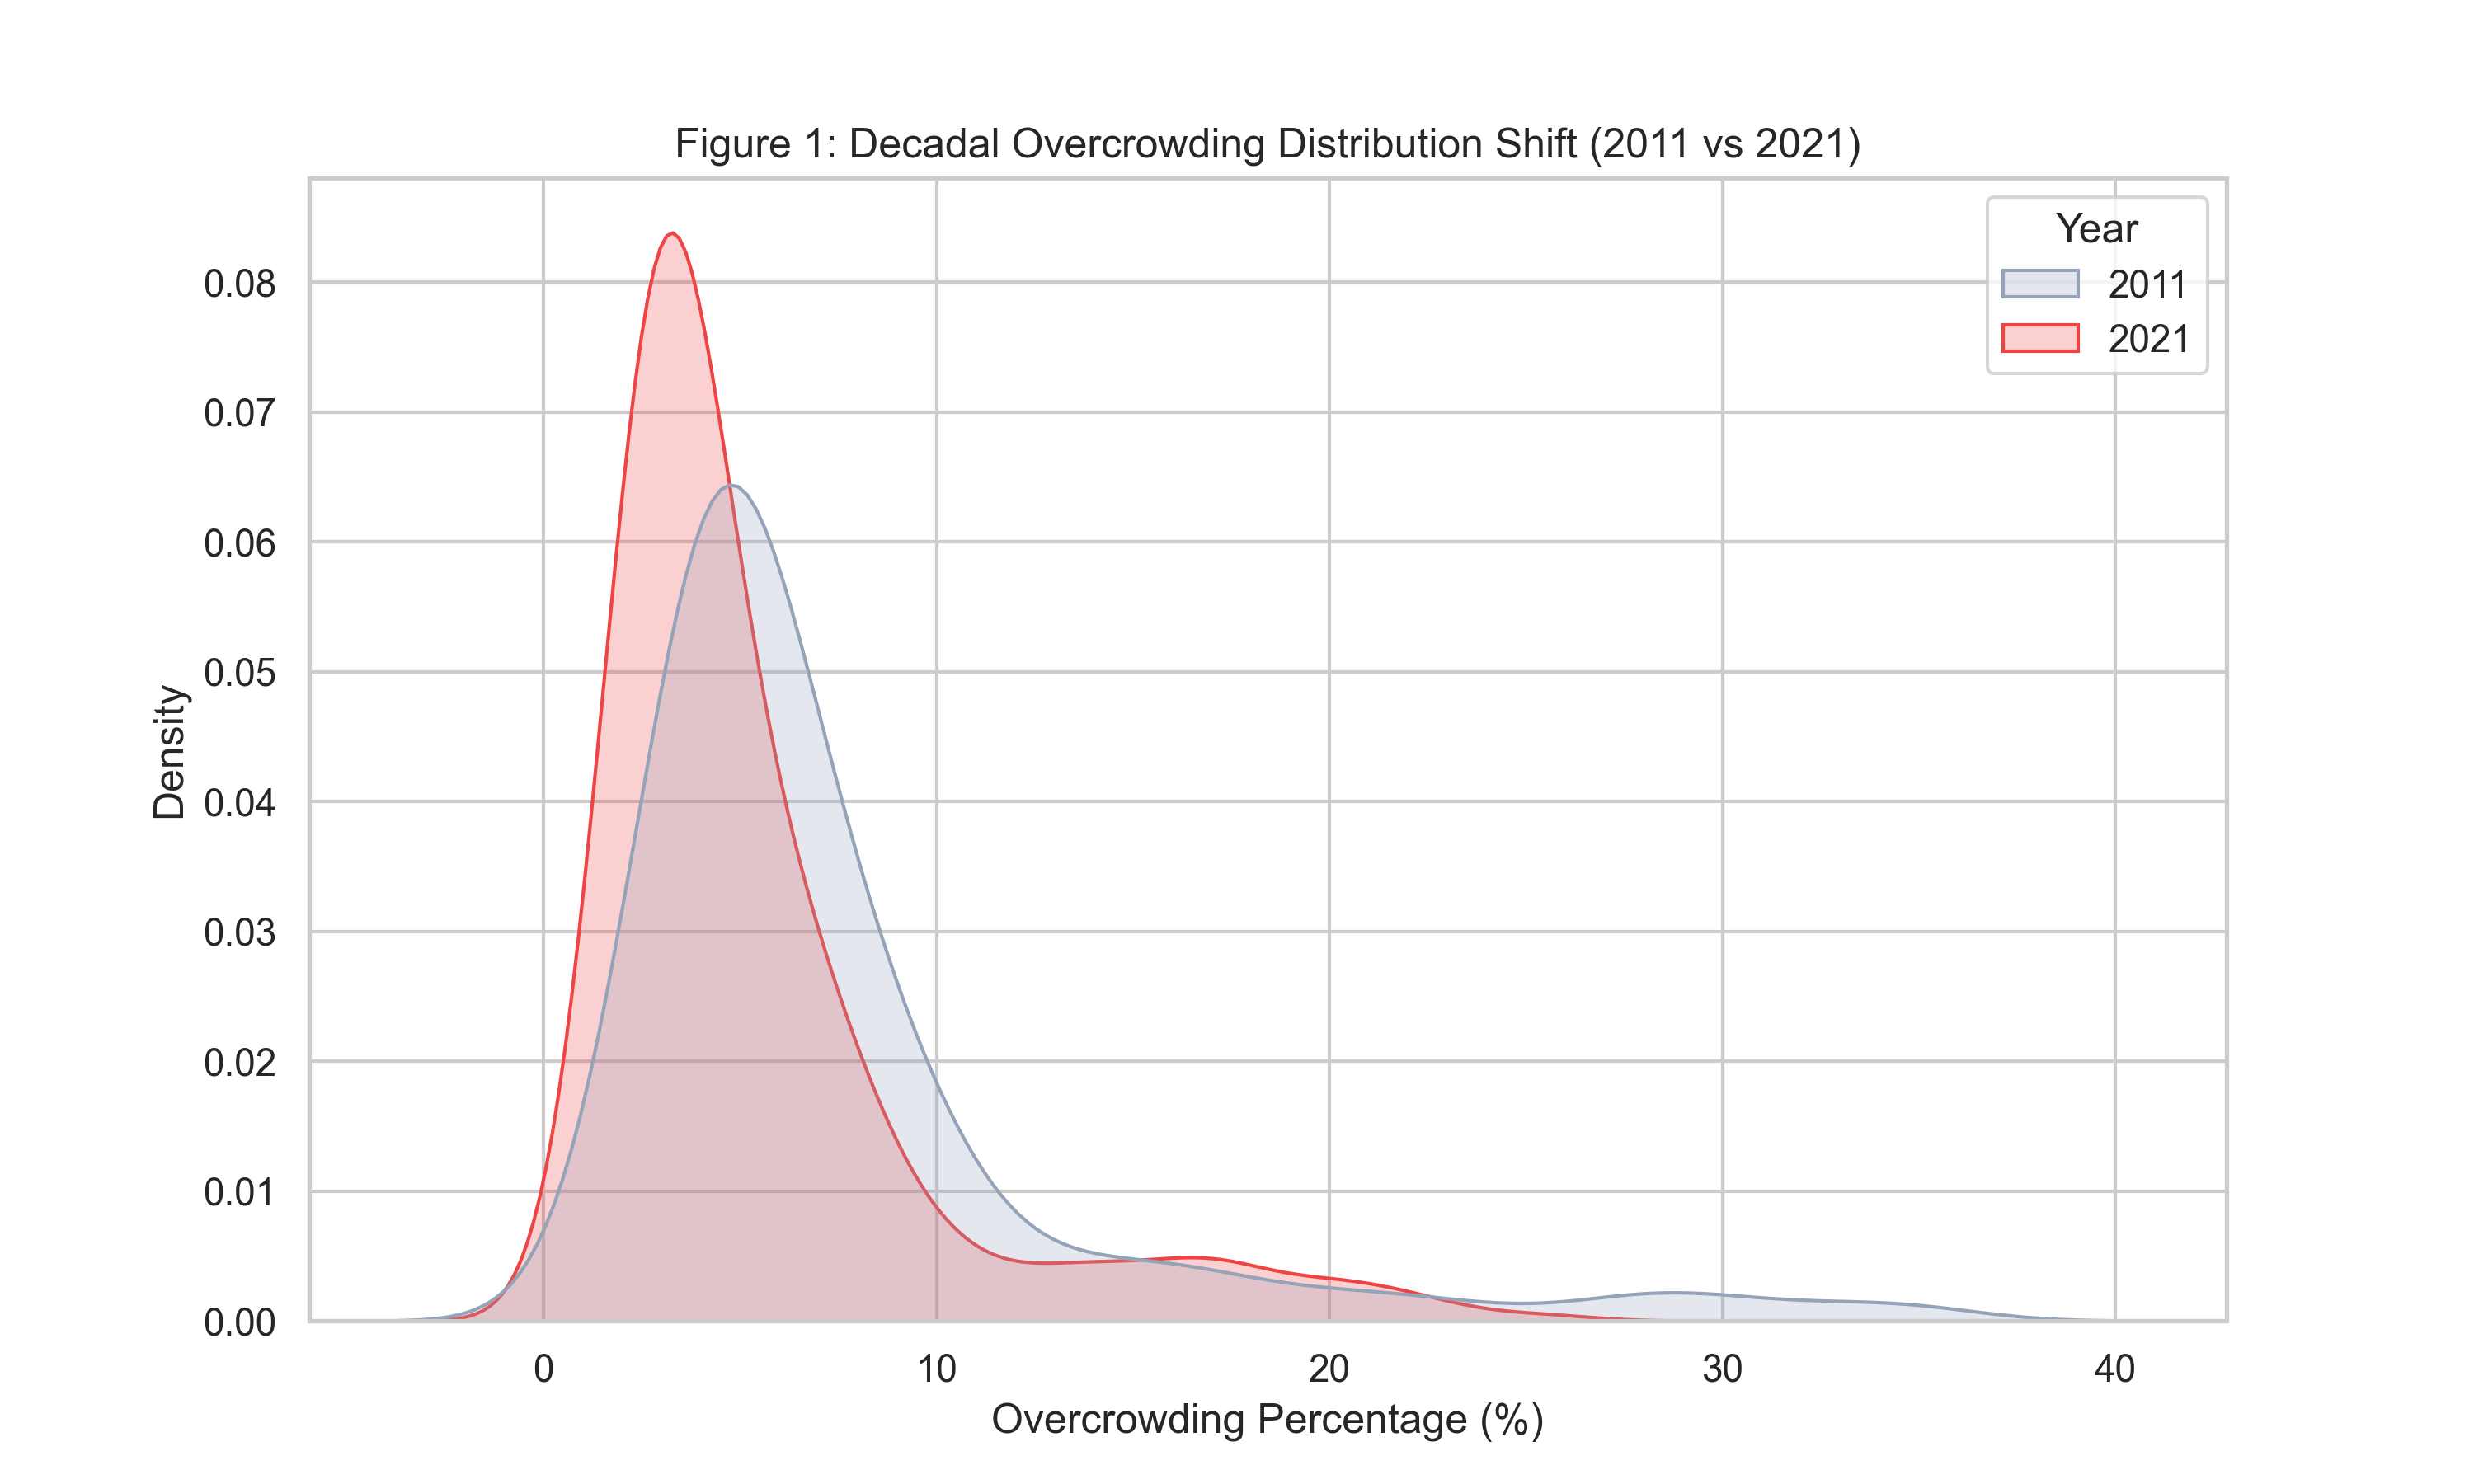
\includegraphics[width=0.45\textwidth]{figures/eda_overcrowding_shift.png}
    \caption{Decadal Overcrowding Distribution Shift (2011 vs 2021): Highlighting the compression and redistribution of housing pressure across the UK.}
    \label{fig:overcrowd_shift}
\end{figure}


\subsection{Relationship Analysis: Regression Scatterplots}
Scatterplots with regression lines were used to analyse the relationship between home ownership and overcrowding. This design supports correlation detection and outlier identification simultaneously. A simple linear trend line helps users interpret the dominant structural pattern while preserving visibility of individual Local Authorities.

The persistent negative relationship observed across both census years demonstrates that regions with lower ownership consistently experience higher overcrowding pressure. This choice is grounded in Munzner’s principle of exposing both aggregate structure and individual observations within the same view\cite{noauthor_visualization_nodate}. Colour was intentionally used conservatively to avoid unnecessary cognitive overload, with emphasis placed on slope and spatial distribution.

\begin{figure}[htbp]
    \centering
    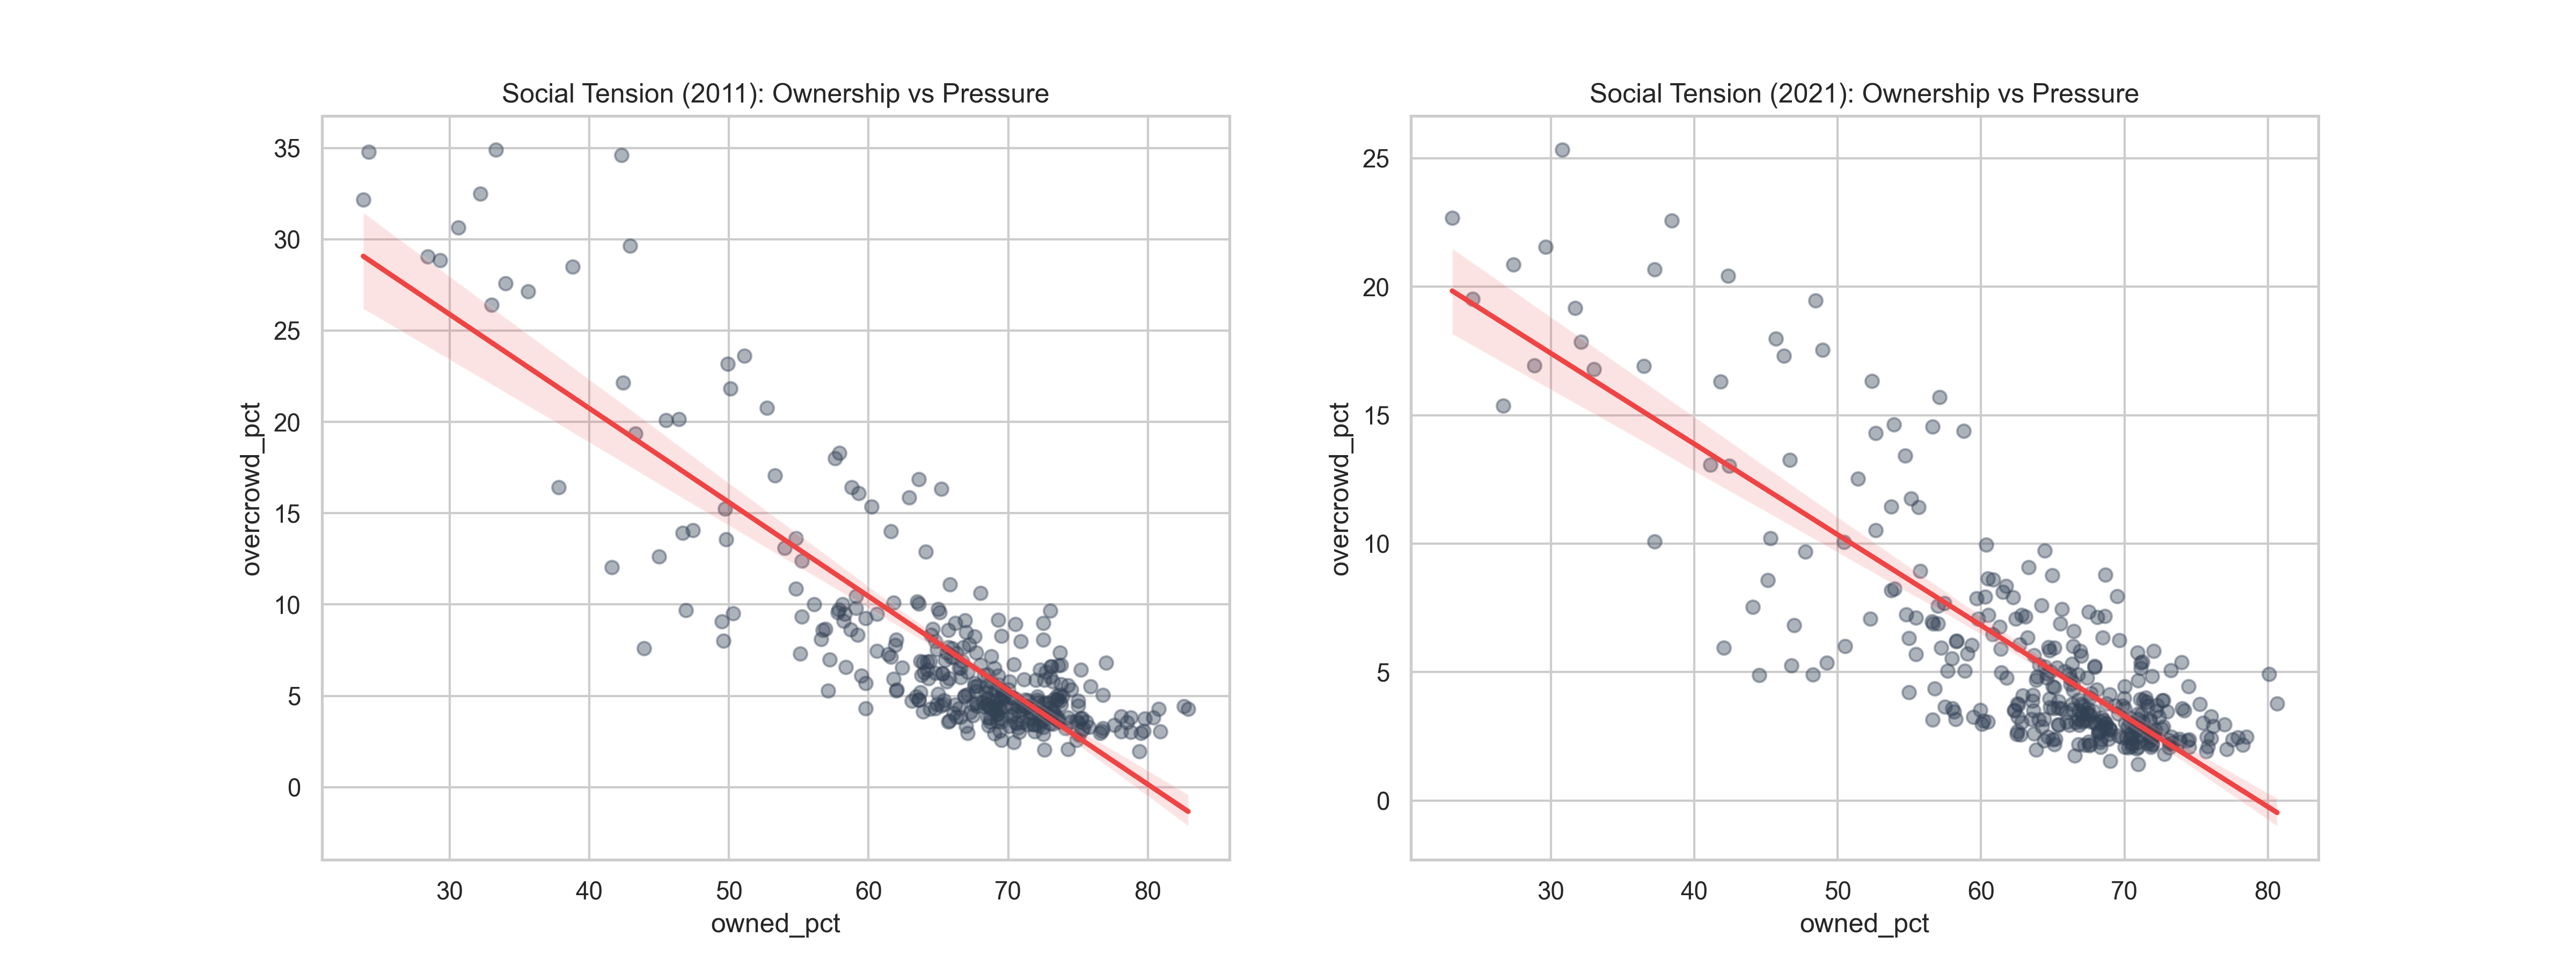
\includegraphics[width=0.48\textwidth]{figures/eda_social_tension.png}
    \caption{Social Tension Analysis: Ownership vs Overcrowding Pressure in 2011 (Left) and 2021 (Right), showing the persistent negative correlation.}
    \label{fig:social_tension}
\end{figure}


\subsection{Correlation Matrix}
A correlation heatmap was used to summarise systemic relationships among housing indicators in 2021. This technique allows users to quickly identify strong positive and negative associations across multiple variables without requiring repeated pairwise scatterplots.

The heatmap shows that overcrowding is strongly positively correlated with high-density housing and private renting, while negatively correlated with ownership. This supports the interpretation that the housing crisis is structurally linked to density concentration and rental market expansion rather than isolated affordability issues. A diverging colour scale centred at zero was used because humans interpret contrast more efficiently when neutral values are visually balanced.

\begin{figure}[htbp]
    \centering
    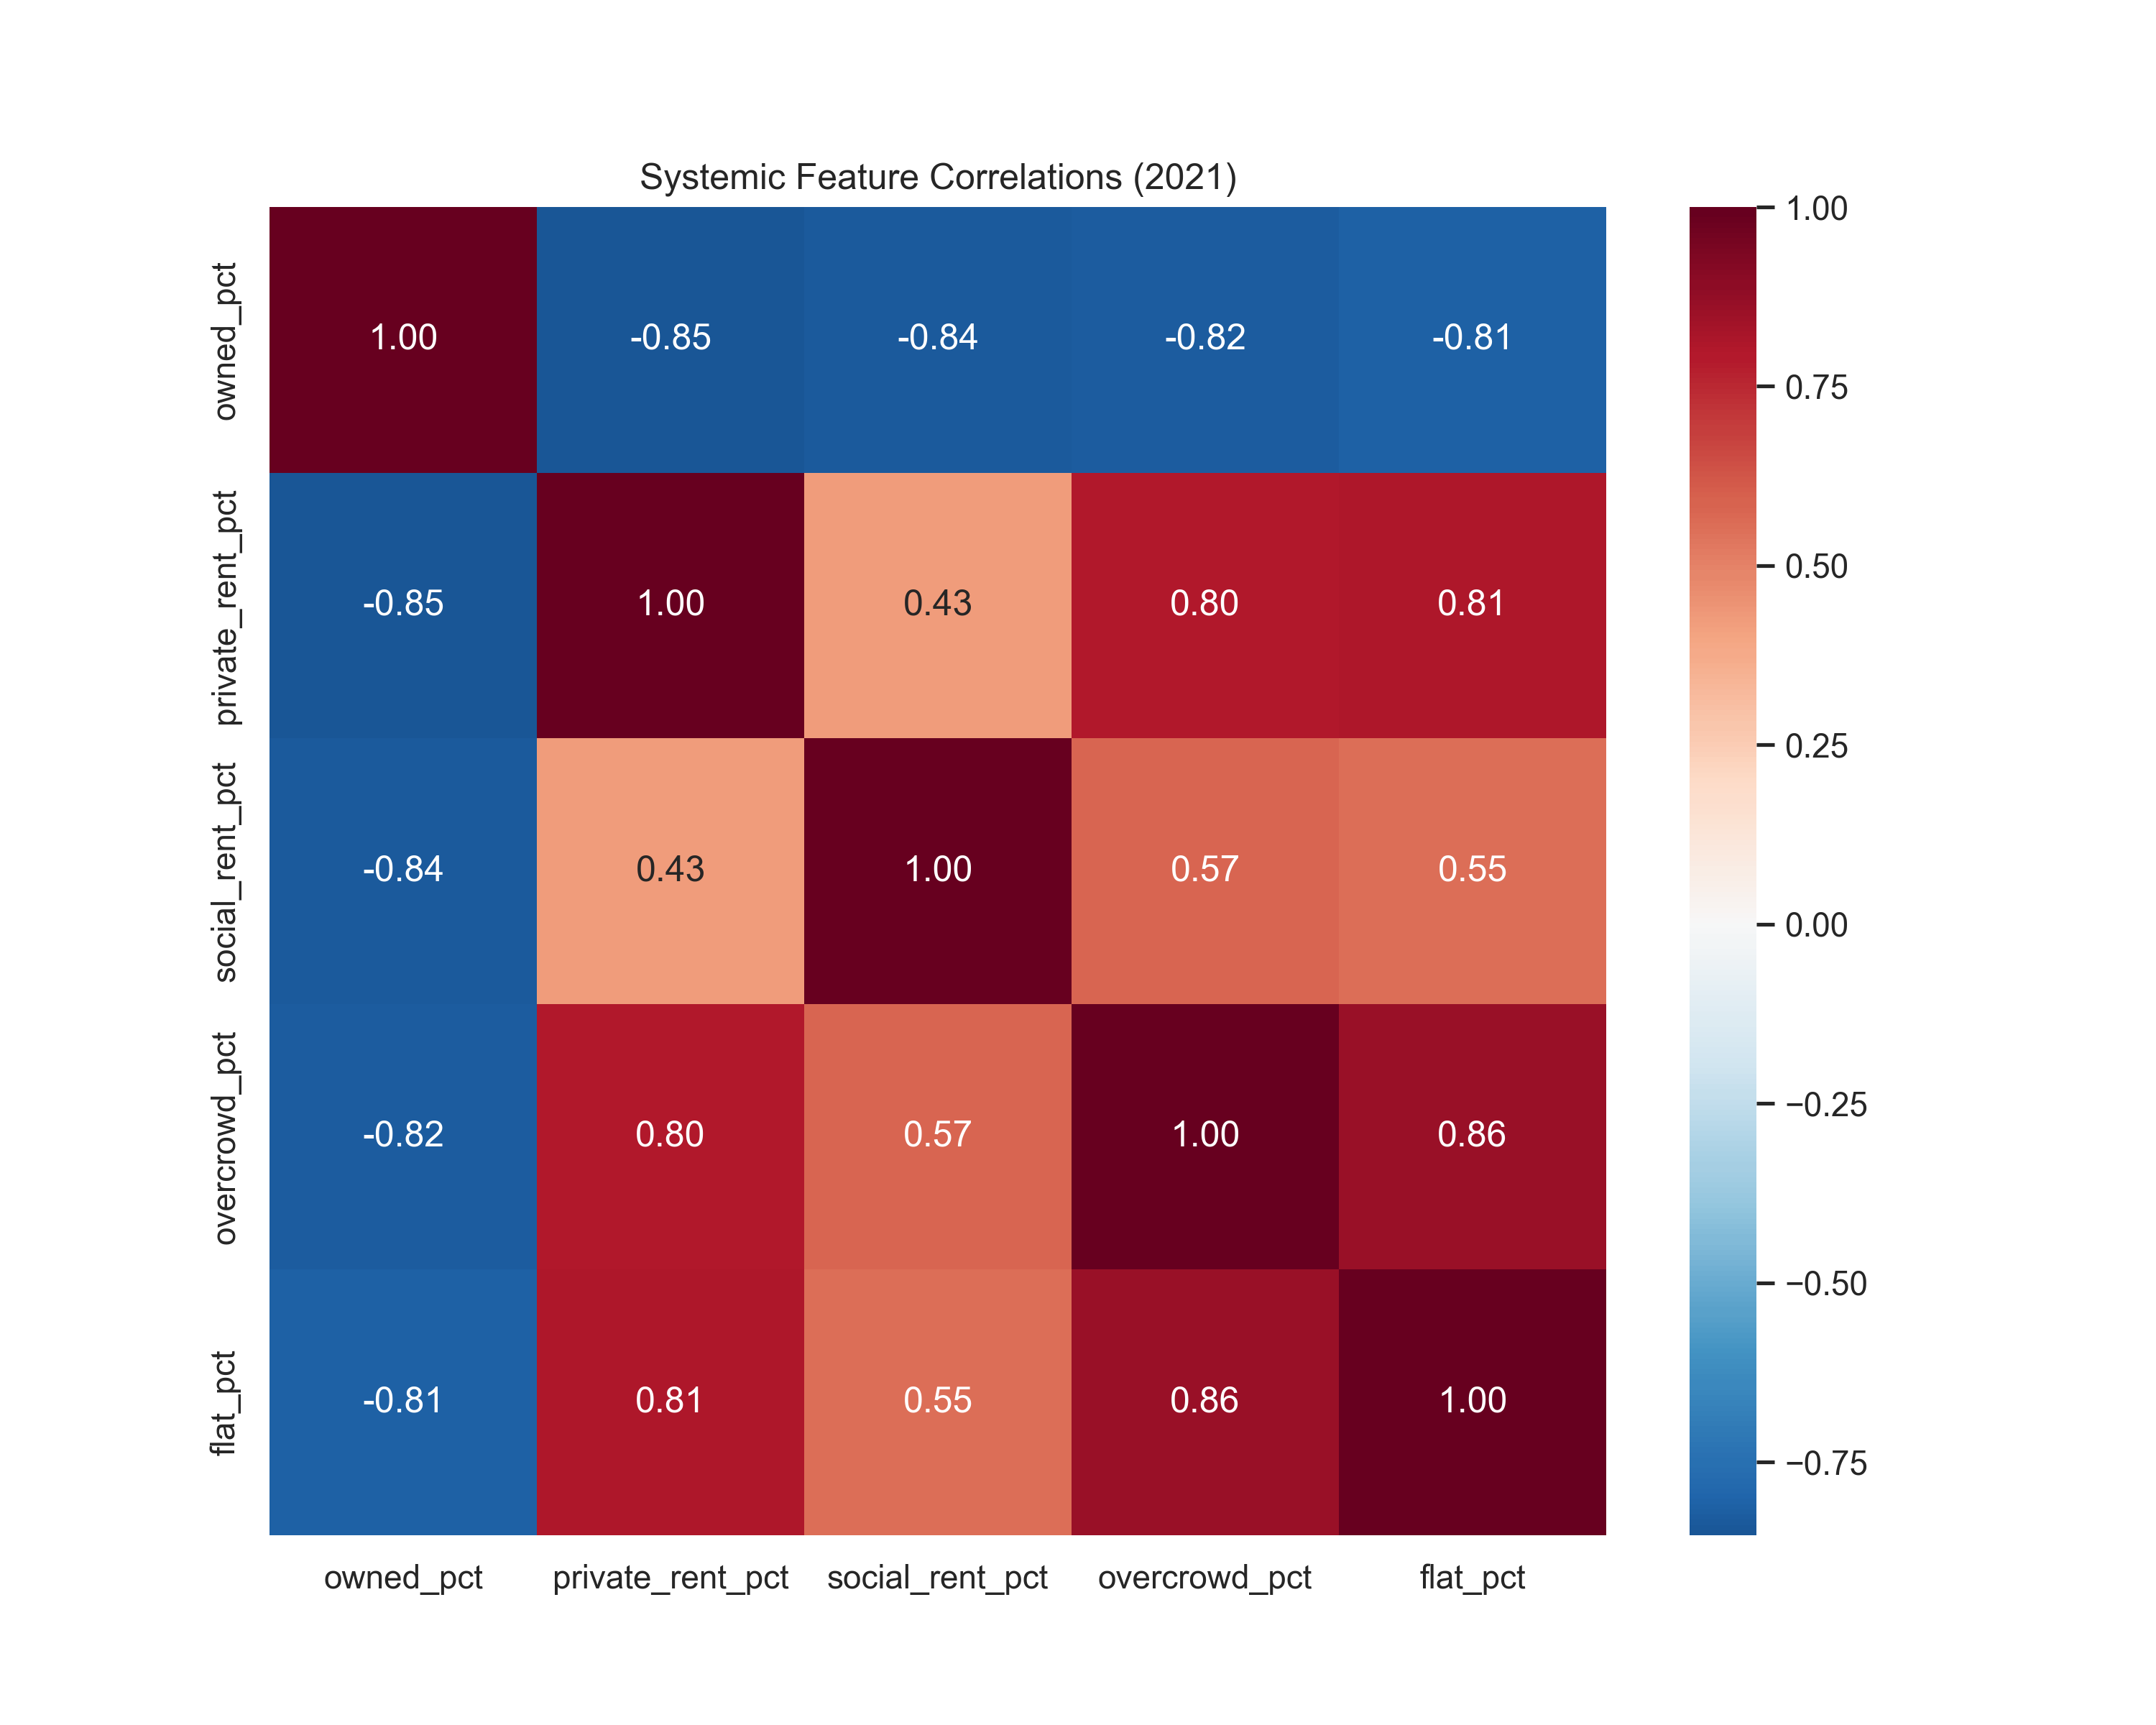
\includegraphics[width=0.45\textwidth]{figures/eda_correlation_matrix.png}
    \caption{Systemic Feature Correlations (2021): Heatmap showing the strong inverse relationship between ownership and overcrowding, and the positive correlation between rentals and pressure.}
    \label{fig:corr_matrix}
\end{figure}


\subsection{K-Means Clustering}
K-Means clustering was applied to identify latent housing archetypes across Local Authorities. This method was selected because the project aims to group structurally similar regions rather than predict predefined labels. Unsupervised clustering allows hidden socio-economic profiles to emerge directly from the data. The selected variables were:
\begin{itemize}
    \item Ownership percentage
    \item Private rental percentage
    \item Social rental percentage
    \item Overcrowding percentage
    \item High-density housing percentage
\end{itemize}
The Elbow Method was used to determine the optimal number of clusters, and four clusters were selected as the best balance between explanatory power and interpretability. The resulting archetypes were: \textbf{Established Suburbanites}, \textbf{Central Urban Stressed}, \textbf{Transitional Renters}, and \textbf{Social and Constrained}. This abstraction significantly reduces cognitive complexity by transforming hundreds of Local Authorities into interpretable socio-economic categories, supporting policy segmentation.

\begin{figure}[htbp]
    \centering
    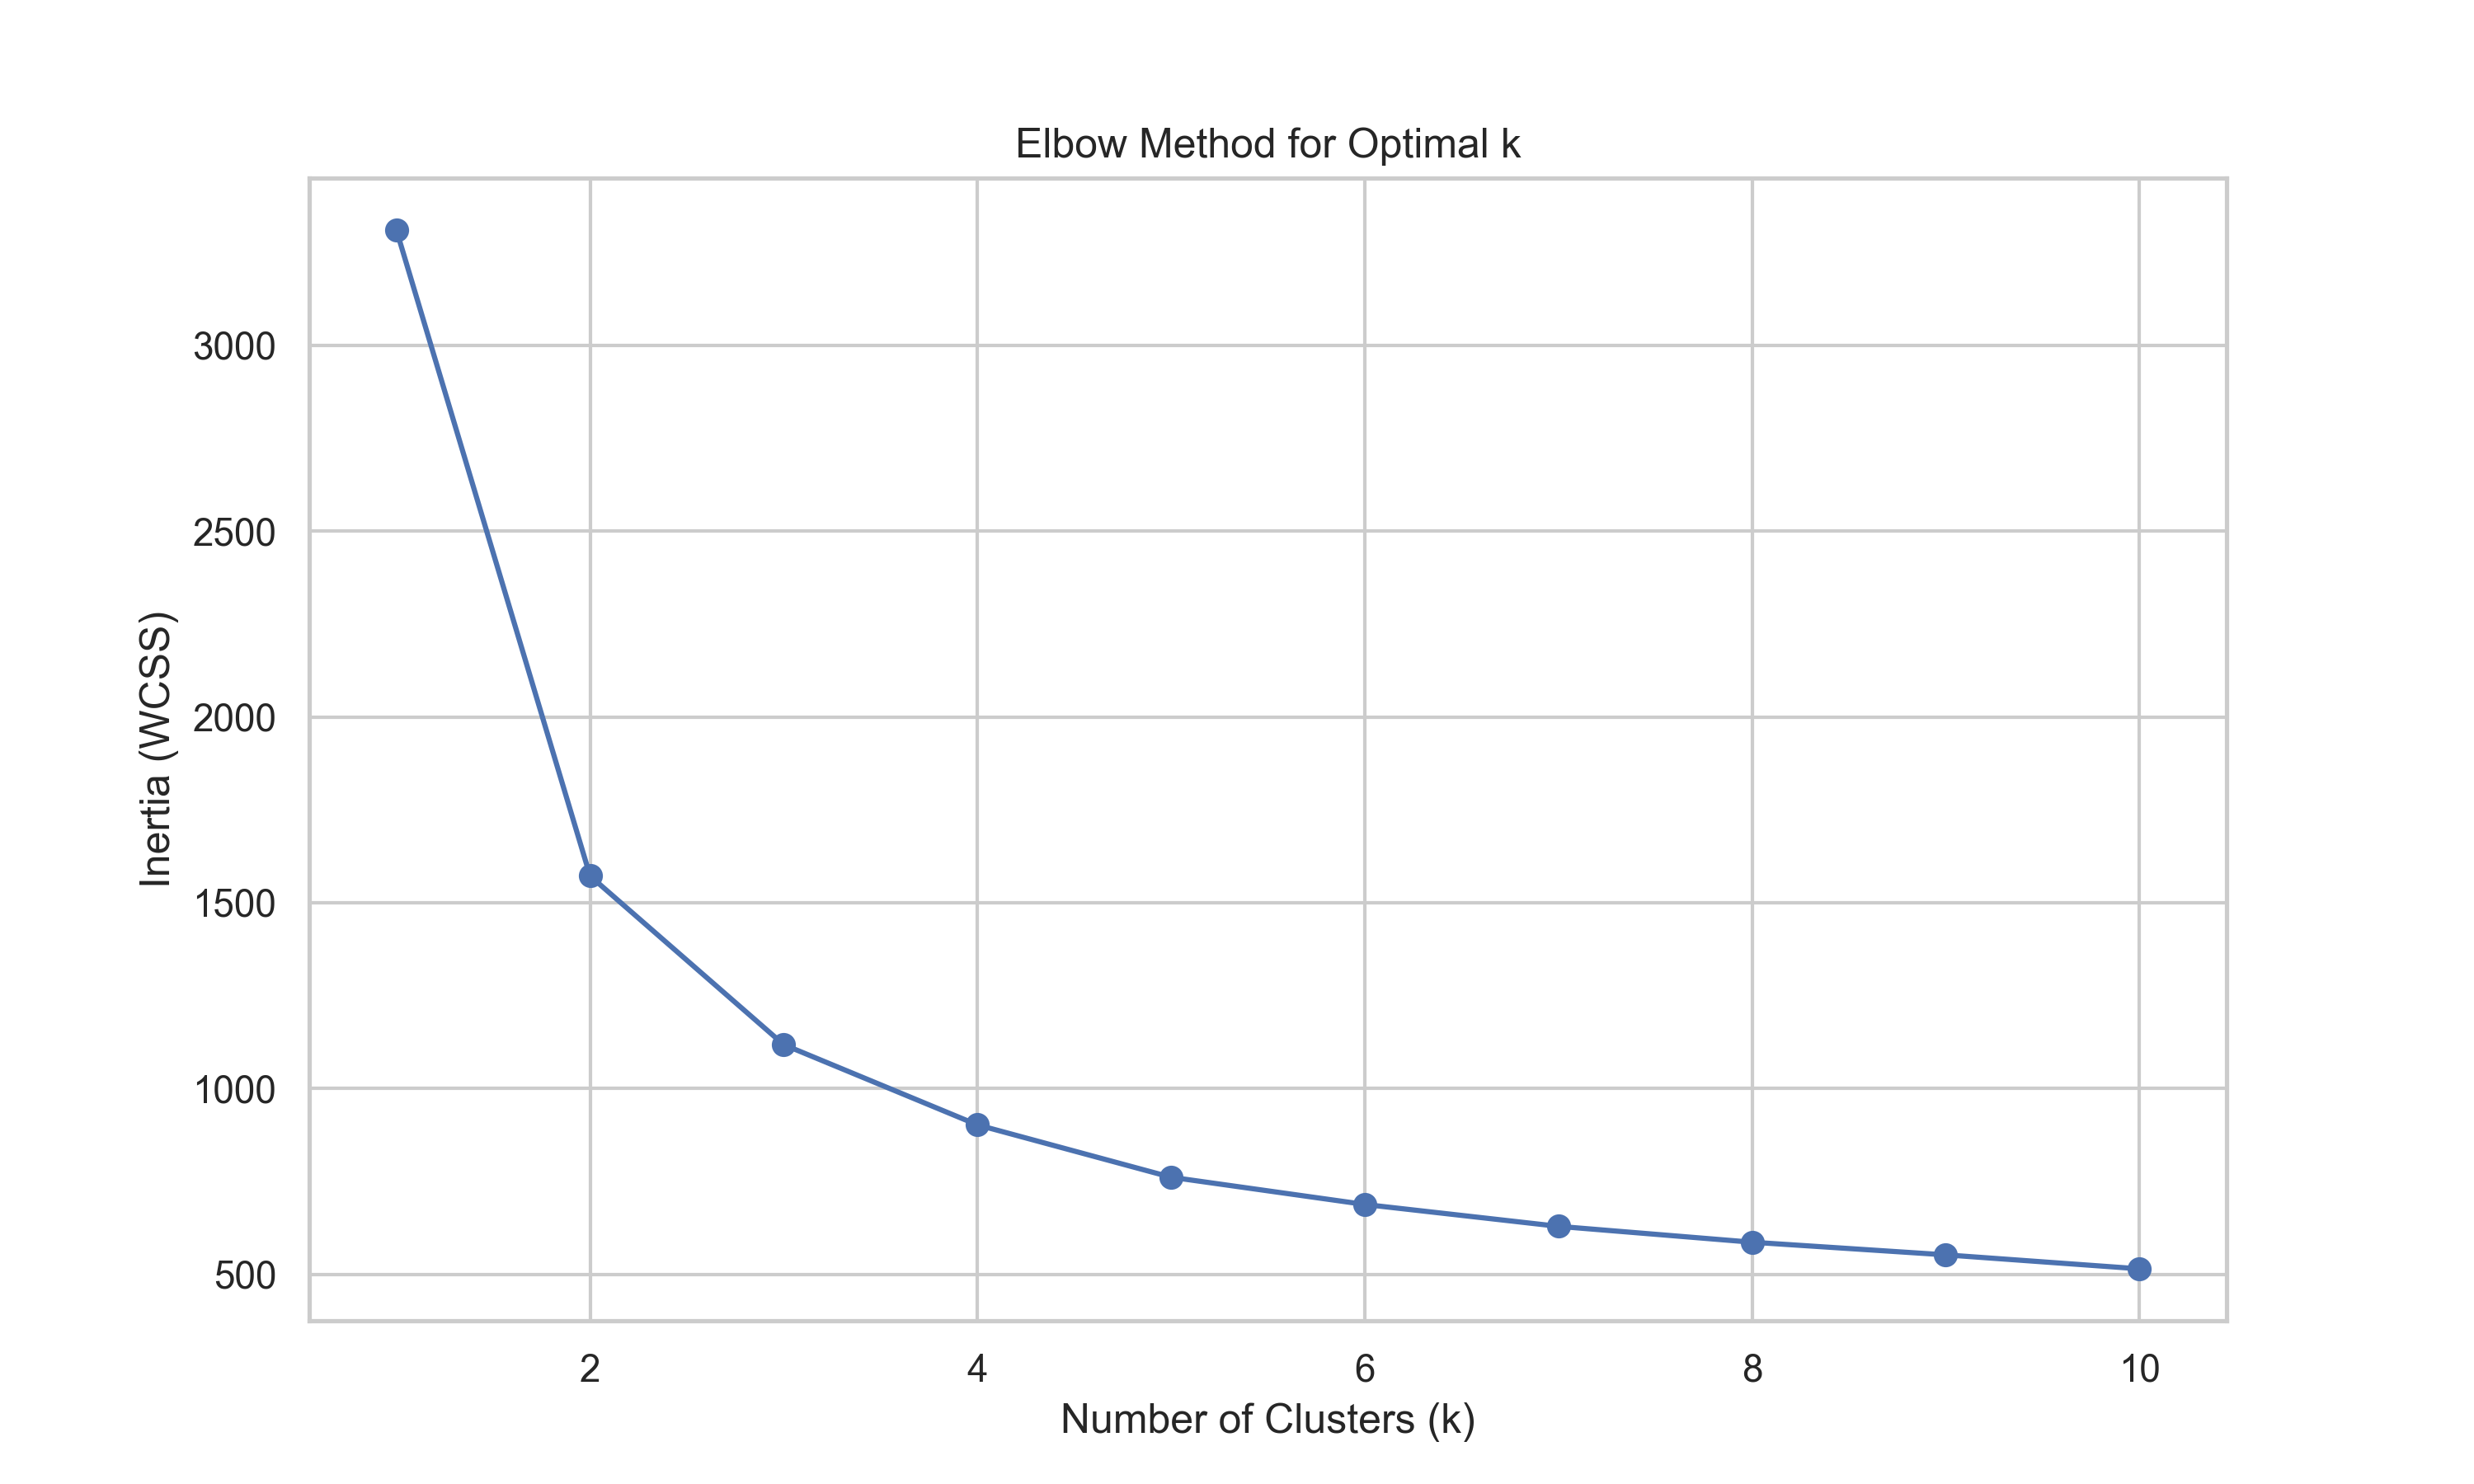
\includegraphics[width=0.48\textwidth]{figures/kmeans_elbow.png}
    \caption{K-Means Elbow Method: Determining the optimal number of clusters by analyzing the reduction in within-cluster sum of squares (WCSS).}
    \label{fig:kmeans_elbow}
\end{figure}


\subsection{Dimensionality Reduction: PCA and t-SNE}
Two projection methods were required by the coursework and were selected for complementary purposes rather than redundancy.

\subsubsection{PCA}
Principal Component Analysis (PCA) was selected to preserve global variance structure and provide interpretability through feature loadings. The first two principal components capture the vast majority of meaningful variation (see Table \ref{tab:imputation_eval} for detailed metrics), suggesting that the housing system has a strong low-dimensional structure.

\begin{table}[htbp]
\centering
\caption{PCA Feature Loadings (PC1 and PC2)}
\label{tab:pca_loadings}
\begin{tabular}{@{}lrr@{}}
\toprule
\textbf{Variable} & \textbf{PC1} & \textbf{PC2} \\ \midrule
Owned \% & 0.495 & -0.181 \\
Private Rental \% & -0.435 & -0.503 \\
Social Rental \% & -0.382 & 0.789 \\
Overcrowding \% & -0.454 & -0.081 \\
Flat \% & -0.462 & -0.292 \\ \bottomrule
\end{tabular}
\end{table}

PC1 was strongly influenced by ownership, overcrowding, private renting, and flat-based housing, suggesting that it represents the primary axis of housing pressure.

While PCA preserves global structure, t-SNE was selected to reveal local neighbourhood relationships and improve cluster separation. Housing systems often contain non-linear relationships that linear projection methods cannot fully capture. t-SNE helps expose these local manifolds and improves visual identification of socio-economic neighbourhoods. This was particularly useful for distinguishing high-pressure urban authorities from transitional rental regions. Figures \ref{fig:pca_tsne_archetypes} and \ref{fig:pca_tsne_pressure} illustrate how these projections effectively separate discovered archetypes and visualize the concentration of housing pressure.

\begin{figure}[htbp]
    \centering
    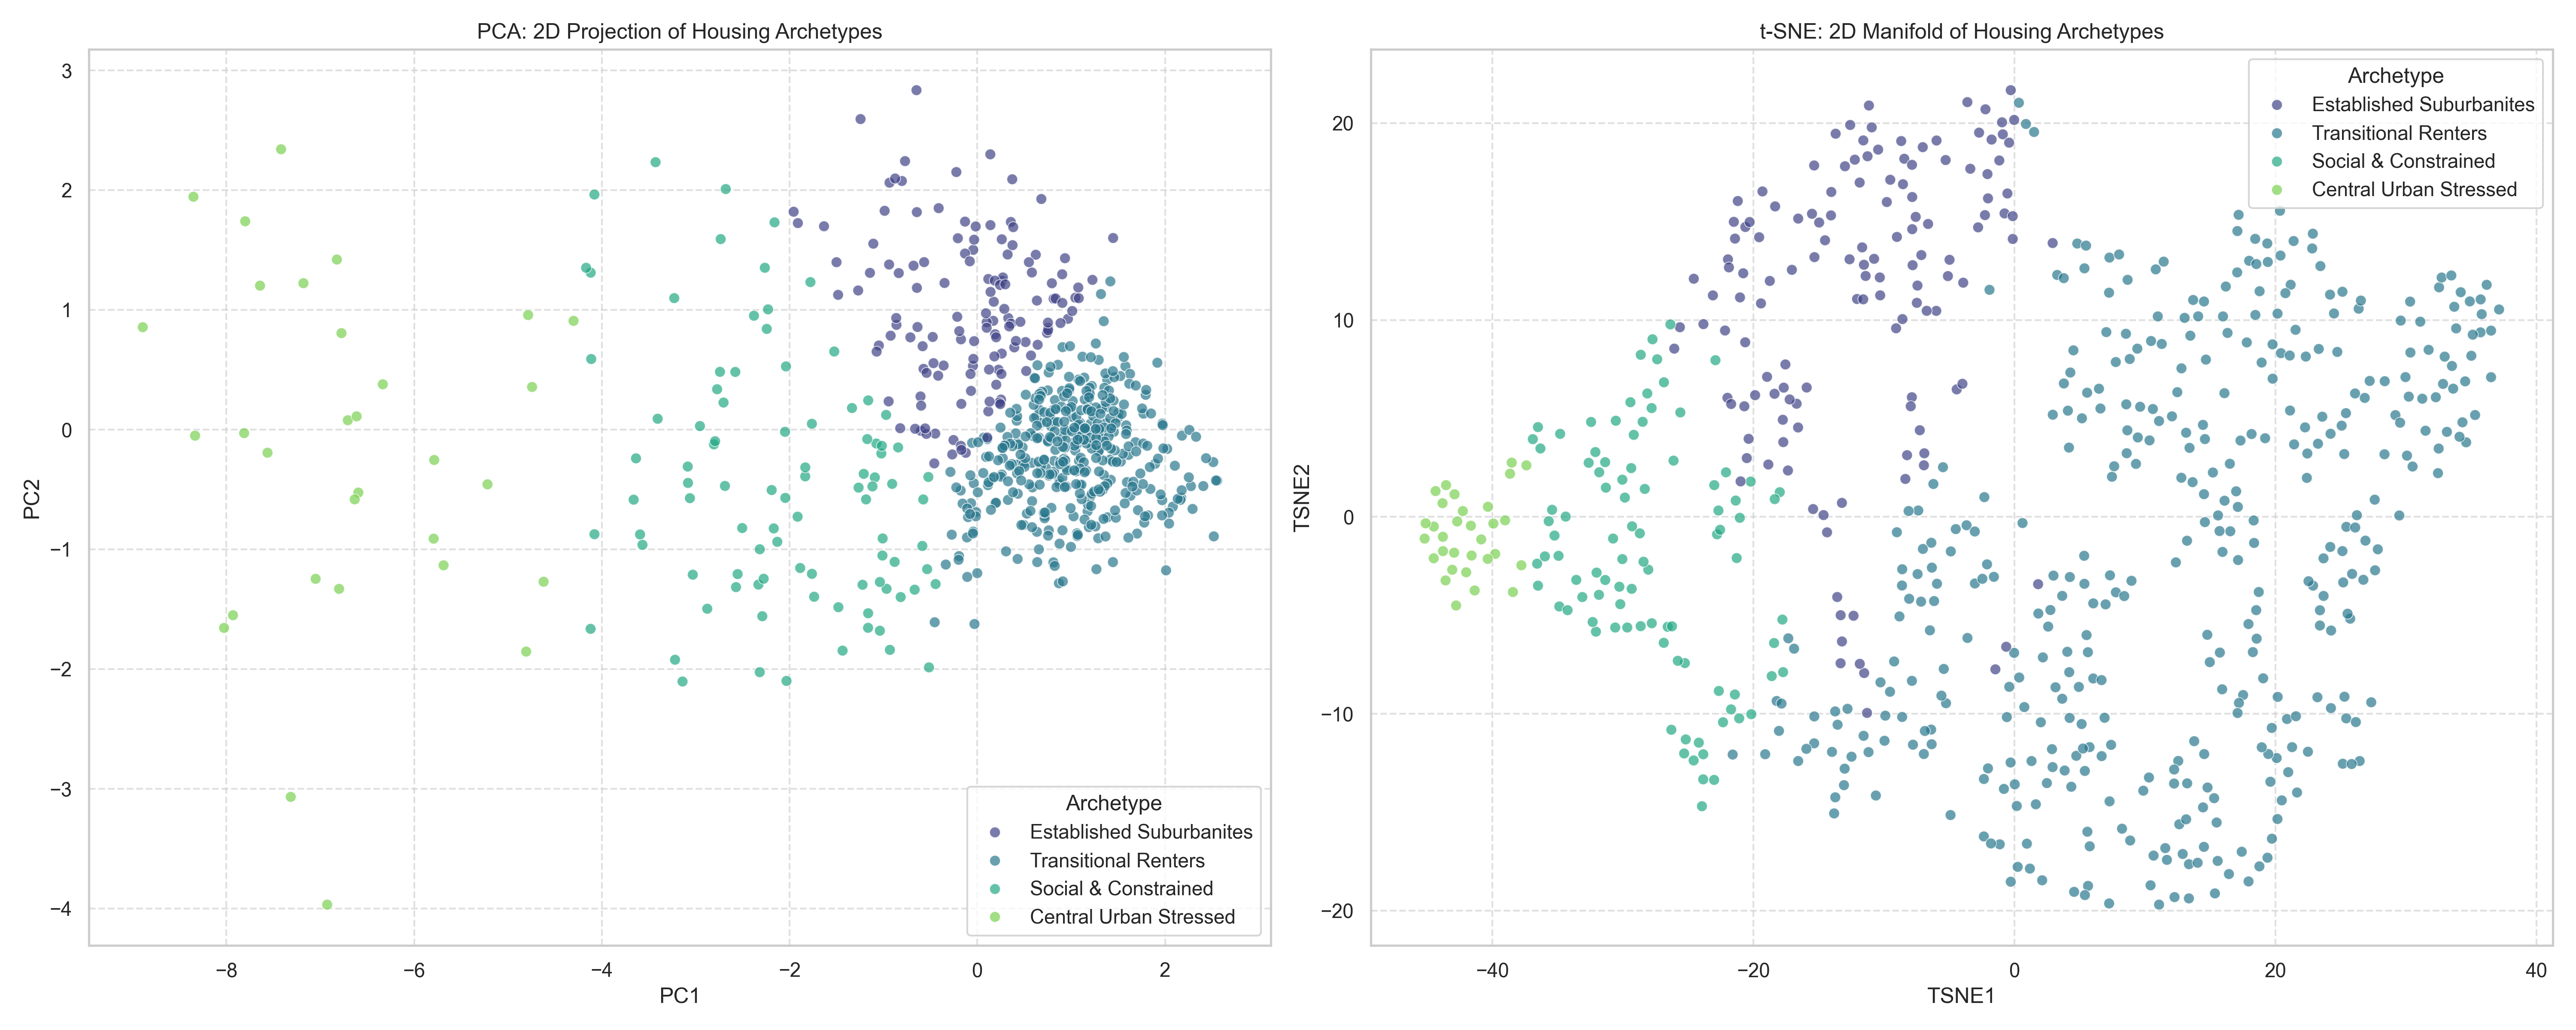
\includegraphics[width=0.48\textwidth]{figures/pca_tsne_archetypes.png}
    \caption{Dimensionality Reduction Comparison (PCA vs t-SNE): Color-coded by discovered housing archetypes, showing cluster separation and global vs local structural representation.}
    \label{fig:pca_tsne_archetypes}
\end{figure}

\begin{figure}[htbp]
    \centering
    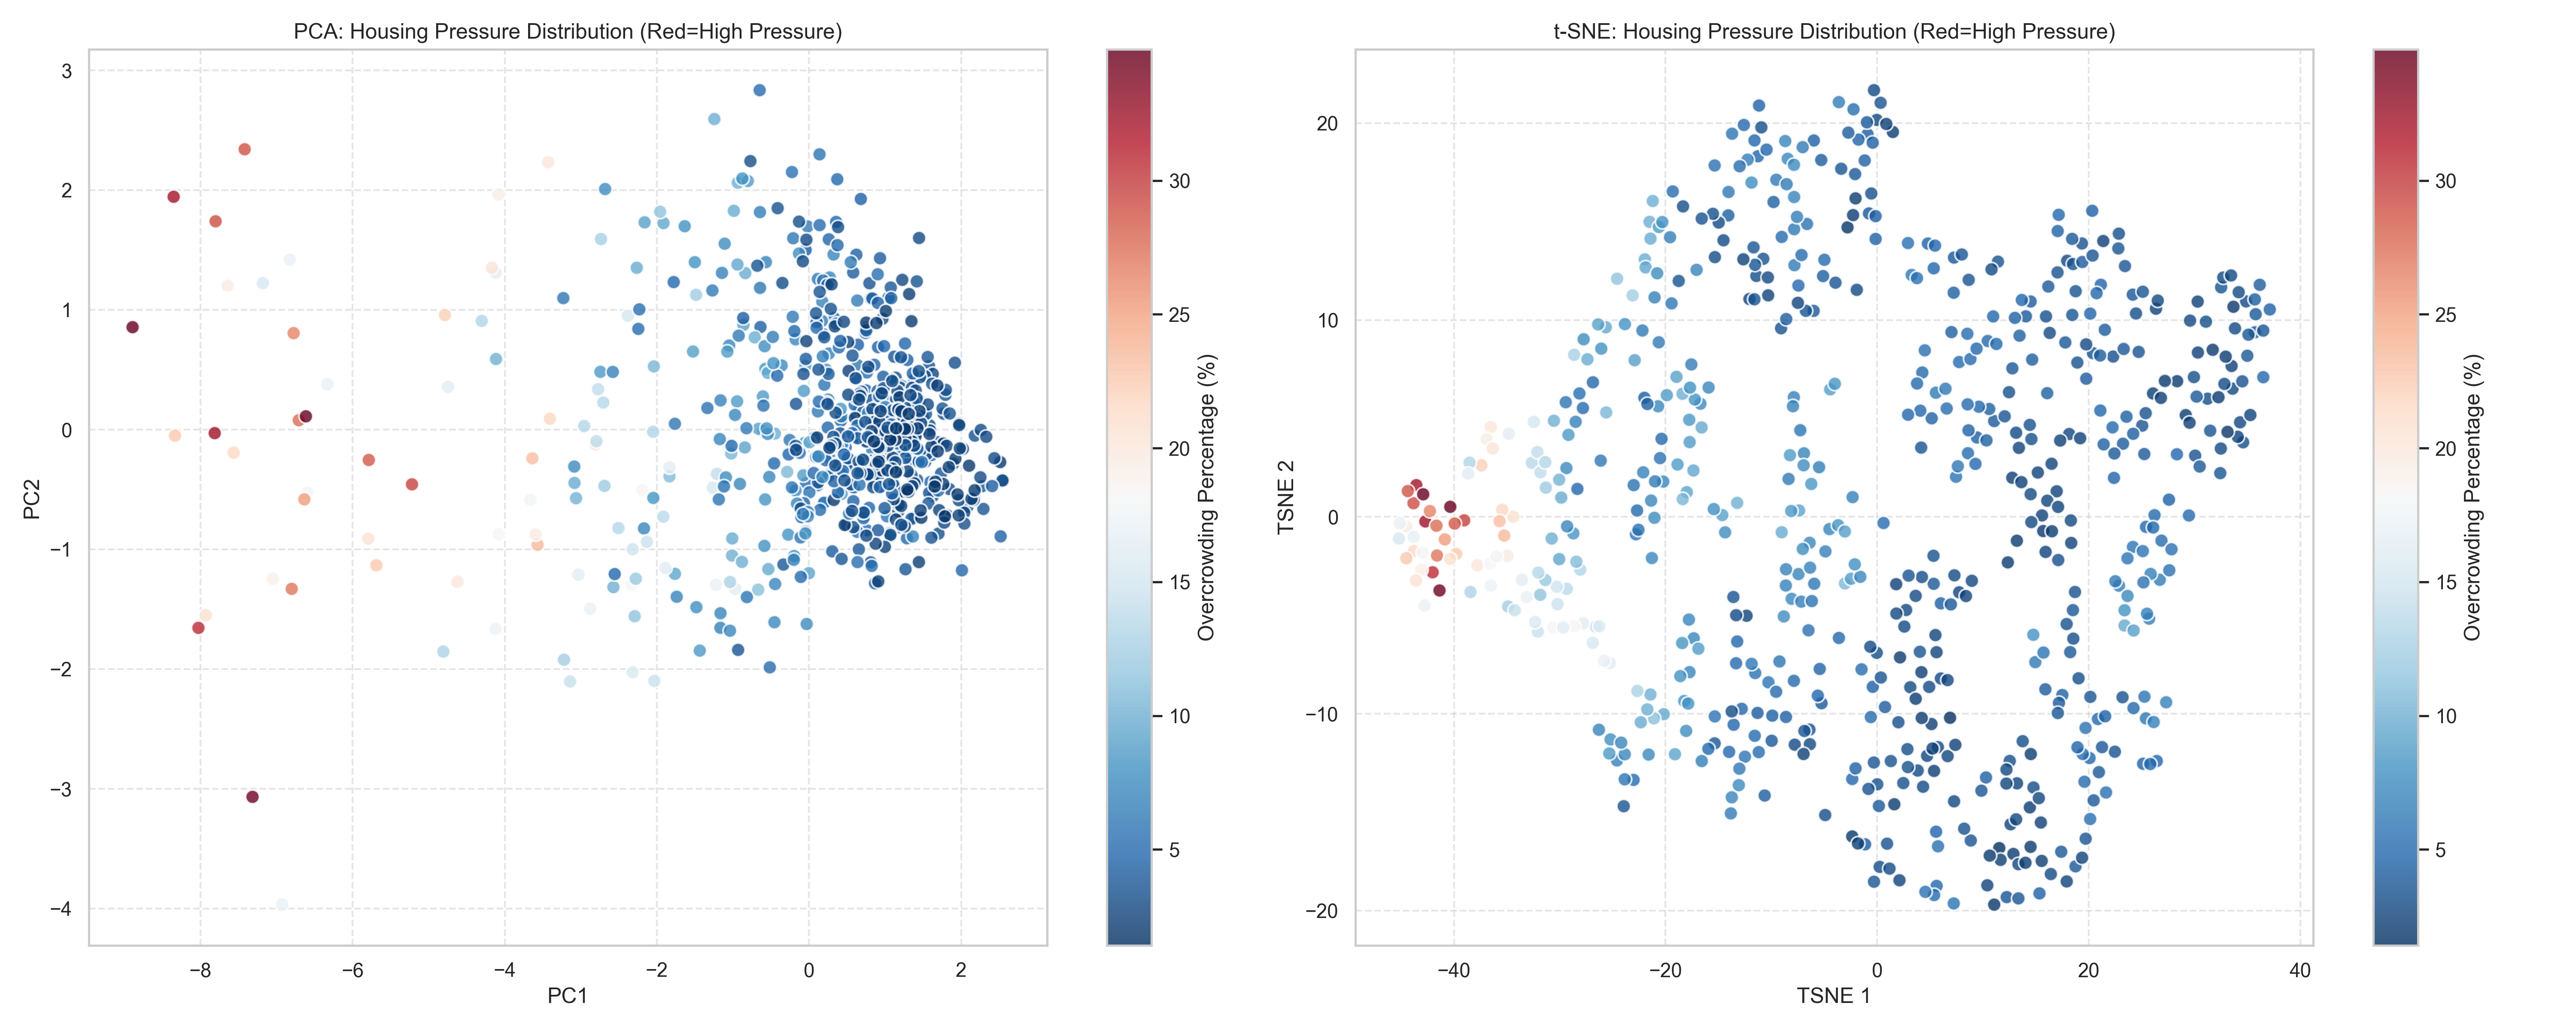
\includegraphics[width=0.48\textwidth]{figures/pca_tsne_pressure_distribution.png}
    \caption{Manifold Projection of Housing Pressure: Heatmap visualization showing the concentration of overcrowding across the latent housing structure.}
    \label{fig:pca_tsne_pressure}
\end{figure}

\subsection{Bayesian Imputation}
Missing values were addressed using Bayesian Ridge Regression to preserve probabilistic relationships between variables. As detailed in the Evaluation section, this method significantly improved data reliability compared to mean imputation, ensuring that subsequent clustering and projection were based on robust inputs.

\subsection{Bayesian Forecasting}
Bayesian Ridge Regression was also used to forecast overcrowding pressure for 2031. Unlike ordinary regression, Bayesian modelling provides posterior uncertainty estimates, allowing decision-makers to evaluate risk. The model uses 2011 structural housing indicators to predict 2021 overcrowding and then projects forward to 2031. The output includes:
\begin{itemize}
    \item Projected overcrowding percentage
    \item 95\% credible intervals
    \item High-risk regional ranking
\end{itemize}
The highest projected pressure was concentrated in regions such as \textbf{Newham}, \textbf{Barking and Dagenham}, \textbf{Slough}, \textbf{Brent}, and \textbf{Haringey}. Uncertainty intervals were visualised using error bars because interval length communicates confidence more effectively than numerical tables alone.

\begin{figure}[htbp]
    \centering
    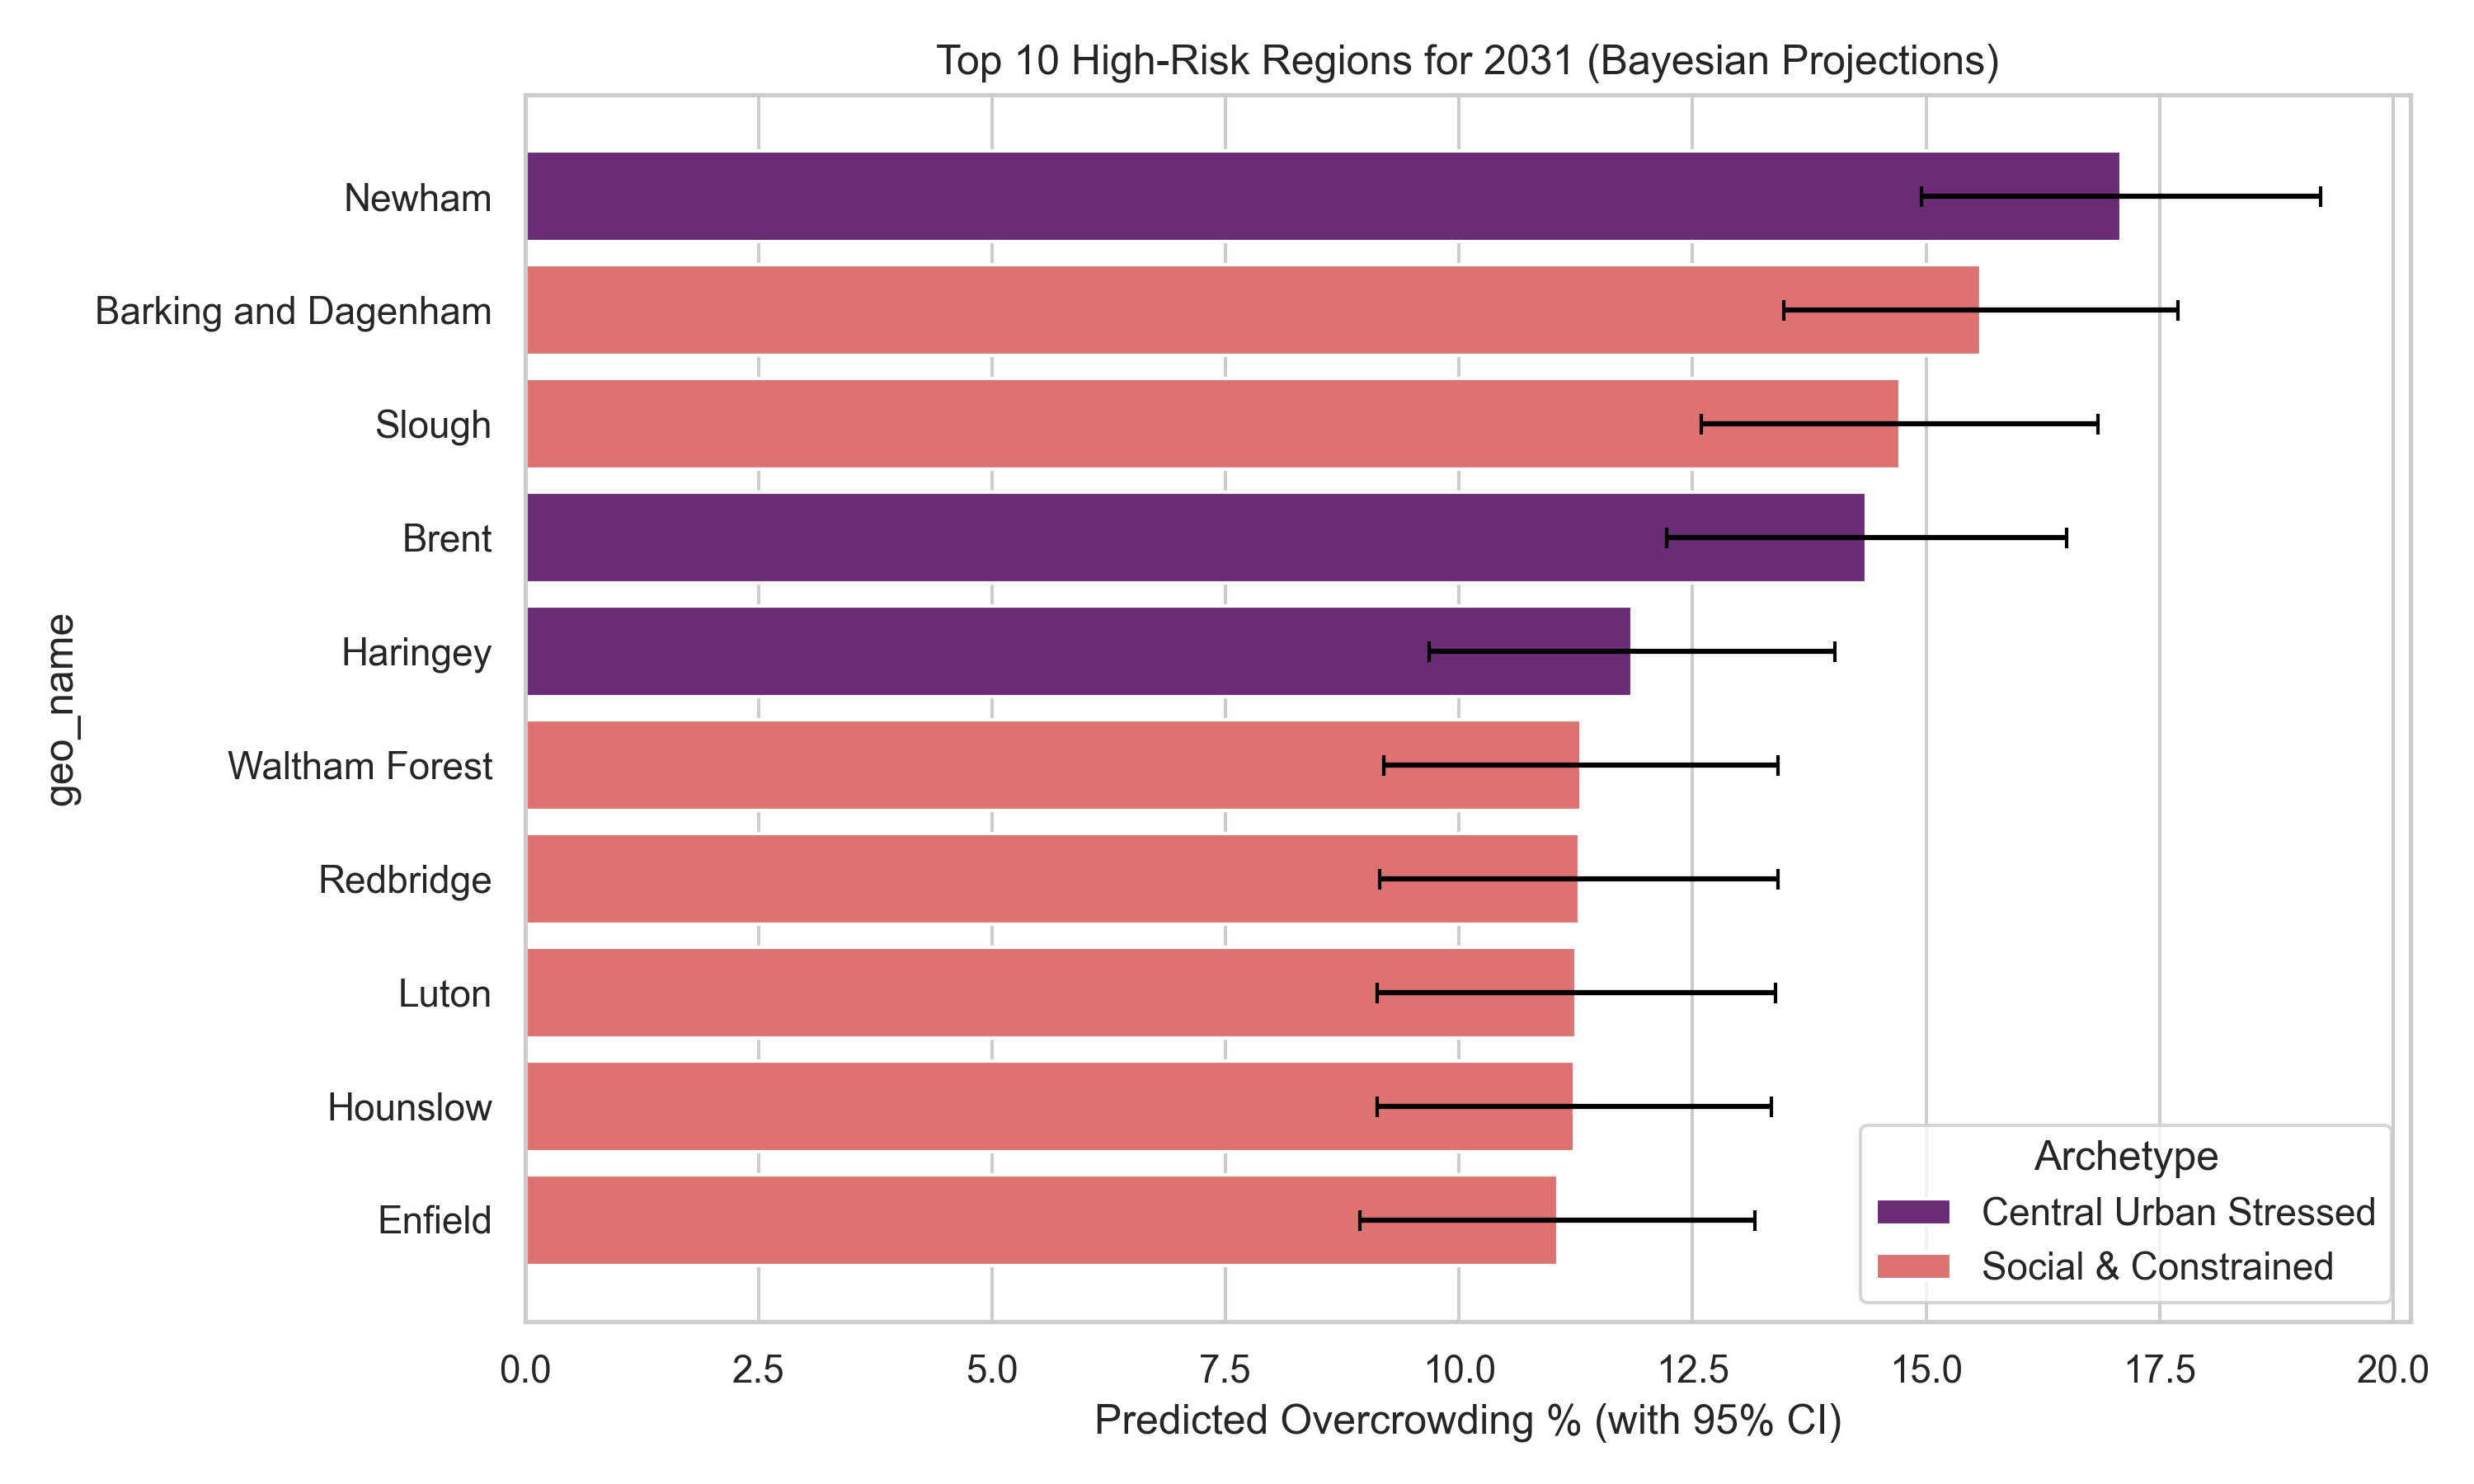
\includegraphics[width=0.48\textwidth]{figures/top_risk_regions.png}
    \caption{Top 10 High-Risk Regions for 2031: Utilizing error bars to communicate Bayesian uncertainty in future overcrowding projections.}
    \label{fig:top_risk}
\end{figure}


\subsection{Tableau Dashboard Design}
The final Tableau dashboard integrates all analytical layers into a single exploratory environment. Users can:
\begin{itemize}
    \item Compare 2011 and 2021 conditions.
    \item Inspect housing archetypes.
    \item Explore PCA and t-SNE projections.
    \item Identify high-risk authorities.
    \item Examine Bayesian uncertainty intervals.
\end{itemize}
Tooltips were included for all projected points so users can identify the corresponding Local Authority immediately. Interactive filtering by archetype and year reduces cognitive overload and supports task-driven exploration. The dashboard therefore functions as an analytical decision-support system.


\section{Evaluation}

\subsection{Evaluation Strategy}
Following Munzner’s nested model for visualisation validation, evaluation was conducted at both the algorithmic level and the user task level\cite{noauthor_visualization_nodate}. This is necessary because a visual analytics system should not only produce statistically reasonable outputs, but also support real users in completing meaningful analytical tasks. Therefore, evaluation was divided into two complementary stages:
\begin{enumerate}
    \item Quantitative validation of modelling choices, including Bayesian imputation quality and projection effectiveness.
    \item Qualitative user evaluation, where students in the discussion group performed analytical tasks using the Tableau dashboard.
\end{enumerate}

\subsection{Algorithm-Level Validation}

\subsubsection{Bayesian Imputation Performance}
The first evaluation focused on missing value handling, since all subsequent clustering and forecasting depend on data quality. A holdout benchmark was created by randomly masking 15\% of complete observations from the 2021 overcrowding variable and comparing predicted values with true values. The benchmark results are shown in Table \ref{tab:imputation_eval}.

\begin{table}[htbp]
\centering
\caption{Benchmark Comparison of Imputation Methods}
\label{tab:imputation_eval}
\begin{tabular}{@{}lrr@{}}
\toprule
\textbf{Method} & \textbf{MAE} & \textbf{$R^2$} \\ \midrule
Mean Imputation & 2.7045 & -0.0941 \\
Bayesian Ridge Imputation & 0.9800 & 0.8476 \\ \bottomrule
\end{tabular}
\end{table}

The Bayesian approach substantially reduced prediction error and produced strong explanatory power, while mean imputation failed to preserve meaningful variance. This confirms that Bayesian imputation is not only theoretically justified but also empirically superior.

\begin{figure}[htbp]
    \centering
    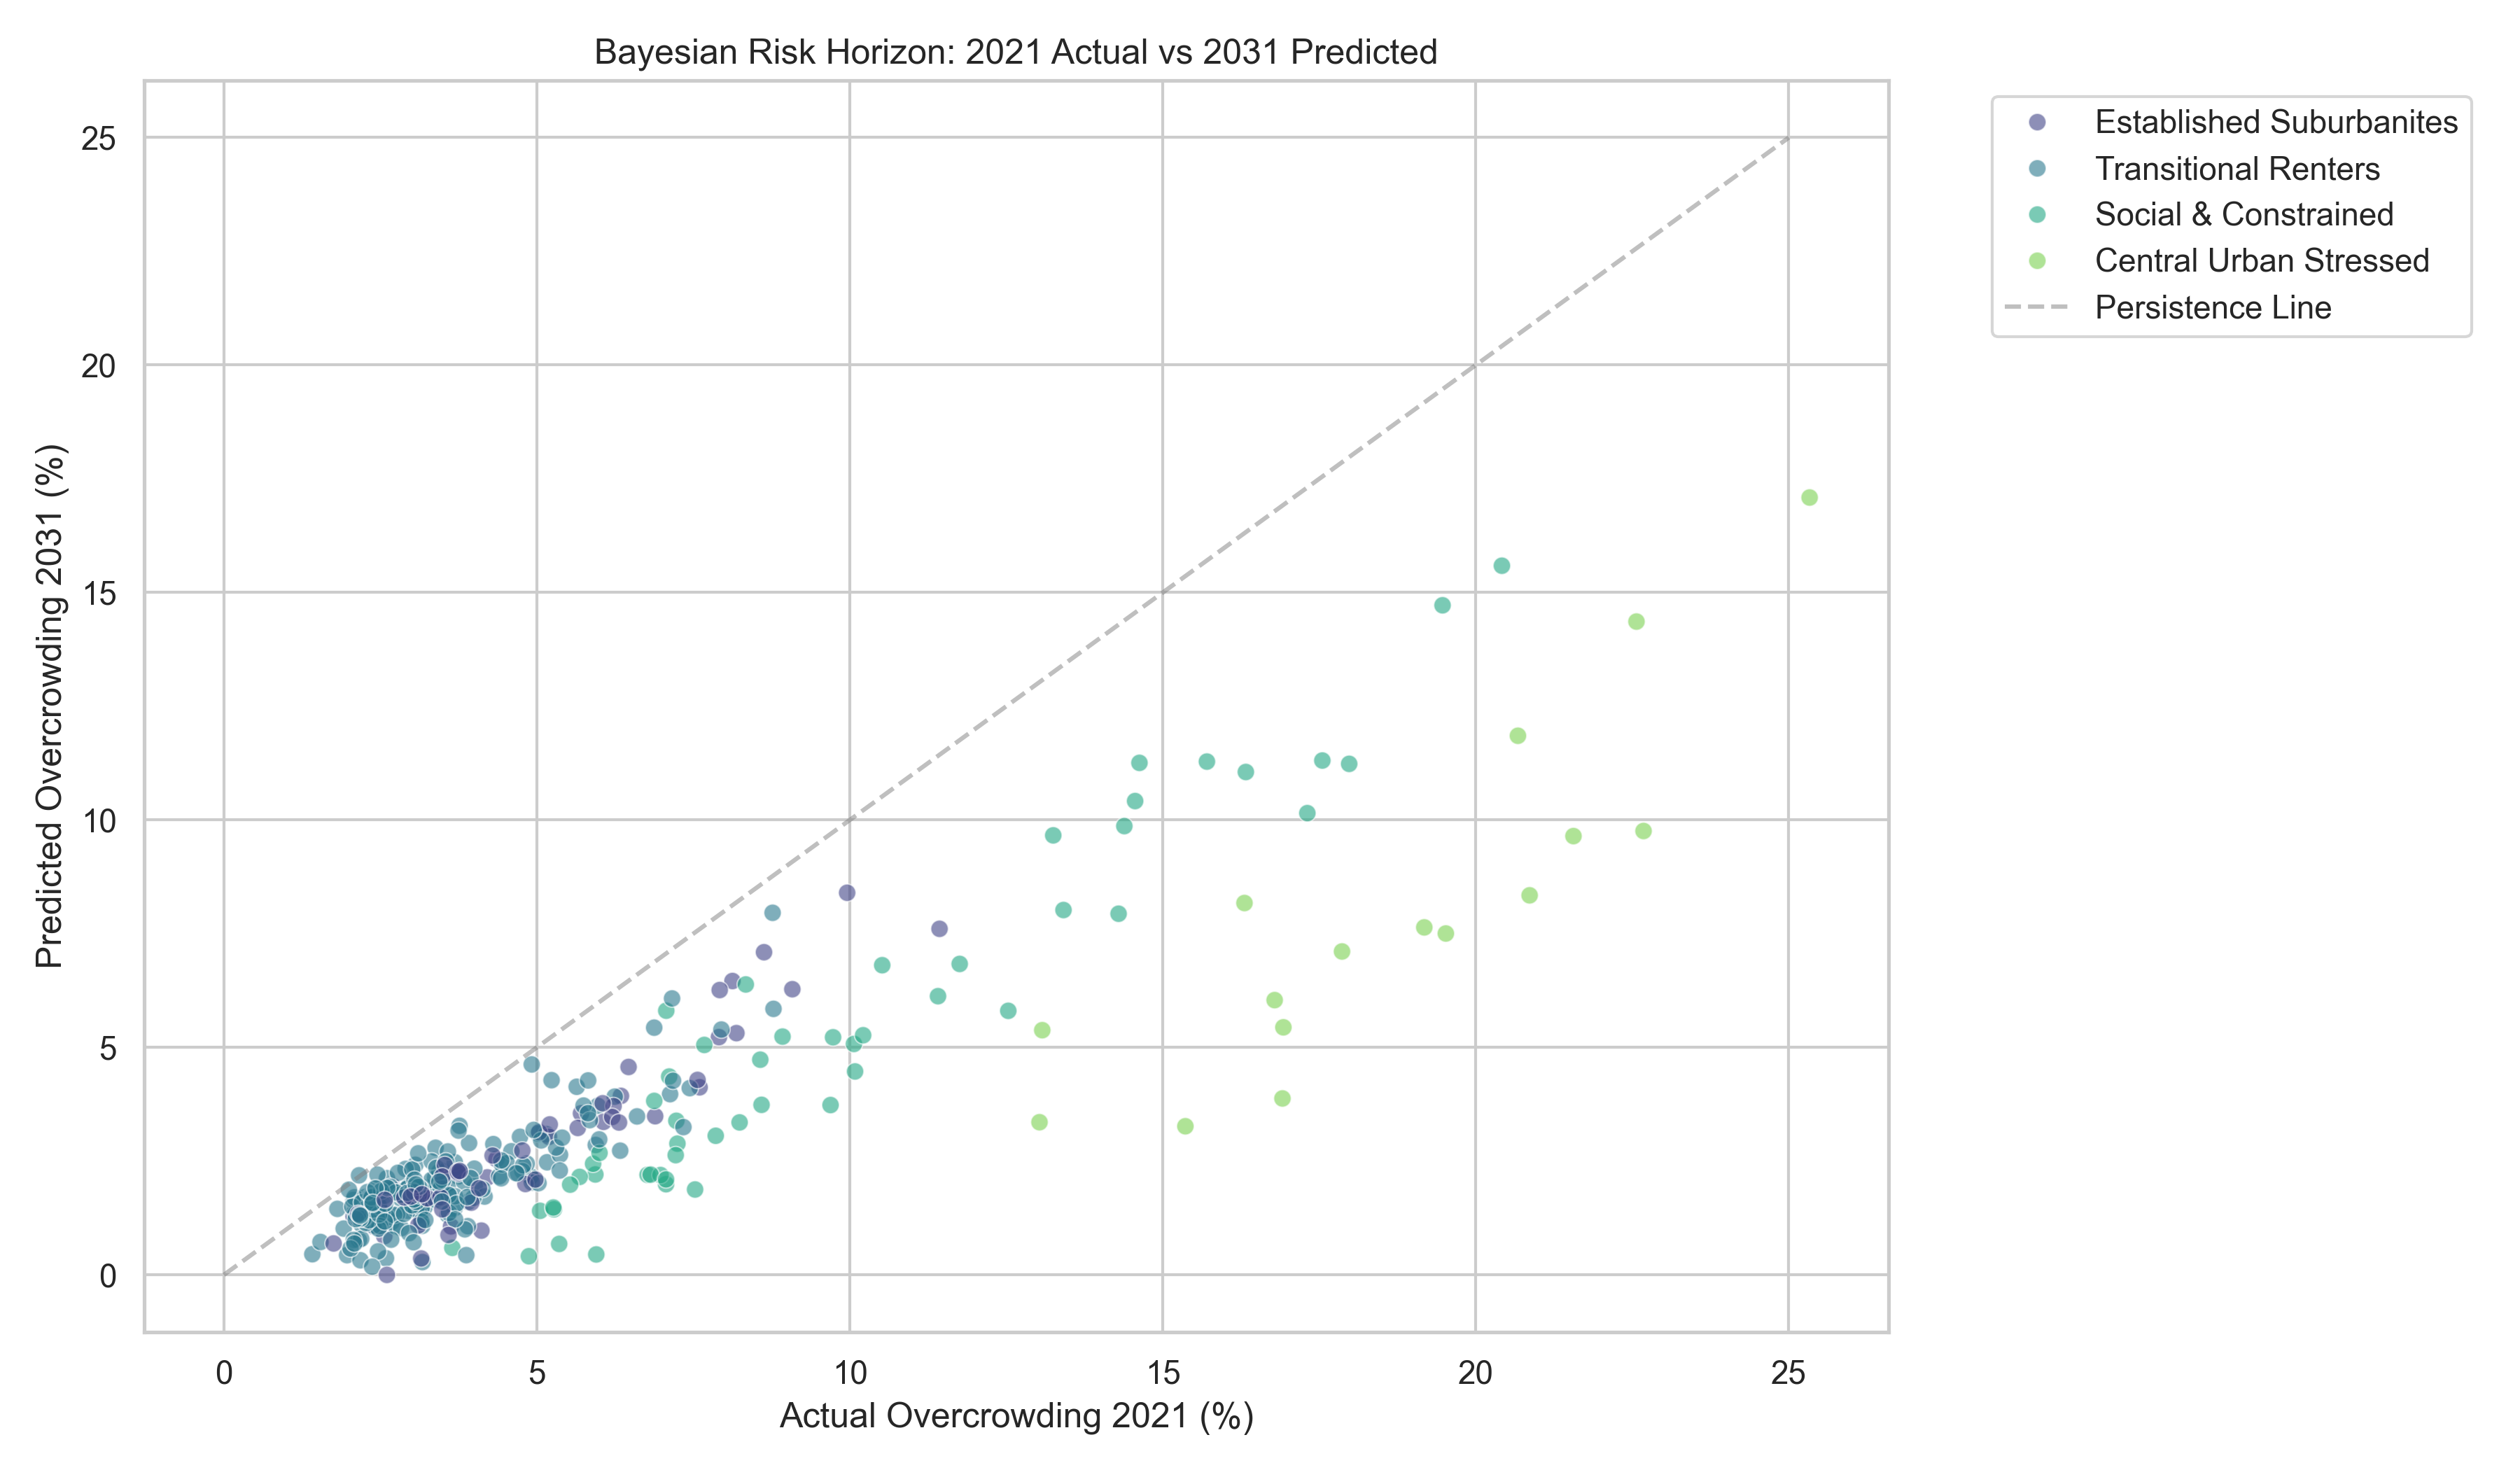
\includegraphics[width=0.48\textwidth]{figures/bayesian_risk_horizon.png}
    \caption{Bayesian Risk Horizon: Comparing 2021 actual overcrowding against 2031 predicted values across discovered archetypes.}
    \label{fig:risk_horizon}
\end{figure}


\subsubsection{Projection Quality}
PCA and t-SNE were evaluated based on structural interpretability and cluster separability. PCA explained 90.8\% of total variance within the first two principal components, indicating that the housing system has strong low-dimensional structure. This high explained variance supports the validity of using two-dimensional projection for dashboard interpretation. PCA loading analysis showed that ownership, overcrowding, private renting, and flat-based housing all contributed strongly to PC1. t-SNE was evaluated visually by comparing neighbourhood separation across housing archetypes, showing clearer local cluster boundaries than PCA for high-pressure urban authorities.

\subsubsection{Clustering Quality}
K-Means clustering was evaluated using both the Elbow Method and interpretability of resulting clusters. Four clusters were selected as they provided a clear reduction in within-cluster variance while maintaining strong semantic interpretability. The resulting archetypes were: \textbf{Established Suburbanites}, \textbf{Central Urban Stressed}, \textbf{Transitional Renters}, and \textbf{Social and Constrained}. Each group showed clear differences in ownership structure, rental dependence, and overcrowding levels.

\subsection{User-Level Evaluation}

\subsubsection{Participants and Tasks}
A qualitative evaluation was conducted with students from the discussion group. Participants were asked to complete several exploratory tasks using the Tableau dashboard without prior explanation of the model structure:
\begin{enumerate}
    \item Identify the Local Authority with the highest projected overcrowding risk.
    \item Compare two regions with similar current overcrowding but different future projections.
    \item Explain the relationship between ownership decline and overcrowding.
    \item Identify which housing archetype represents the highest structural risk.
\end{enumerate}

\subsubsection{Observations}
Most participants were able to complete basic lookup and comparison tasks quickly, particularly when using tooltips and interactive filters. The Top Risk Regions view was considered the easiest to interpret because ranking and uncertainty intervals were visually direct. The PCA projection was generally understood better than t-SNE because users could more easily connect PCA positions to interpretable variables. The housing archetype labels significantly improved comprehension, confirming that semantic naming is essential for policy-facing dashboards.

\subsubsection{Identified Limitations}
Several usability limitations were identified. First, users requested stronger map-based geographic context. Second, users wanted clearer explanations of Bayesian uncertainty intervals. Third, too many simultaneous visual elements increased cognitive load for first-time users. These observations suggest that future versions should improve onboarding and interaction flow.

\subsection{Reflection on Validation Levels}
According to Munzner’s validation framework, this project primarily applies algorithm validation, domain problem validation, and user task validation. For coursework-level evaluation, the combination of quantitative model benchmarking and qualitative analytic task testing provides strong evidence that the system is both methodologically sound and practically useful.

\section{Conclusion}
This study developed a machine learning-driven visual analytics framework to investigate structural housing pressure across Local Authorities in England and Wales using 2011 and 2021 Census data\cite{noauthor_census_nodate}. Rather than treating overcrowding as an isolated housing statistic, the analysis examined its relationship with broader socio-economic structures, including ownership decline, private rental expansion, and high-density residential development.

The results reveal a clear structural transition in the housing system. Overcrowding increased systematically between 2011 and 2021, concurrent with declining home ownership and expanding rental dependency. K-Means clustering and projection analysis effectively distilled these patterns into interpretable archetypes. Bayesian modelling ensured data reliability through imputation and provided policy-relevant forecasts for 2031, complete with uncertainty intervals. This project underscores that effective visual analytics requires careful alignment between user tasks, data abstraction, and modelling choices.

\bibliographystyle{IEEEtran}
\bibliography{references-visa}
\end{document}